\chapter{Digital Electronic Circuits}\label{chap6}

\section*{Introduction}

Digital Electronics is a branch of electronics which deals with Zeros and Ones. A digital circuit responds to only two states of input namely a HIGH and a LOW. A high state corresponds to logic 1 and a low state to logic 0. Logic gates are the basic building blocks of digital circuits and are designed to obey a special algebra called boolean algebra. A digital computer is basically a digital system which comprises of digital circuits.

This Chapter begins with the various number systems and goes on to discuss the different logic gates. It also discusses the simplification of Boolean Expressions, NAND, NOR realisation and adders. The basics of Flip-flops has also been covered at the end of this chapter.

\section{Computer}\label{sec6.1}

The two main categories of computers are
\begin{itemize}
\item[(i)] The Analog Computer

\item[(ii)] The Digital Computer
\end{itemize}

\subsection{Analog Computer}\label{sec6.1.1}
\index{Analog Computer}

Computers use voltages or currents to represent numbers in order to perform computations. An Analog Computer can accept, process and output continuous analog voltages. For example, an analog computer capable of reading 0\,V to 10\,V, can read and understand any voltage value between 0\,V and 10\,V. Analog computers are also referred to as linear systems. For example, an analog adder can add two voltages say 3.2\,V and 2.4\,V representing numbers 3.2 and 2.4 and give the sum as 5.6\,V representing number 5.6 as shown in the block diagram of Fig.~\ref{fig6.1}. 
\begin{figure}[H]
\centering
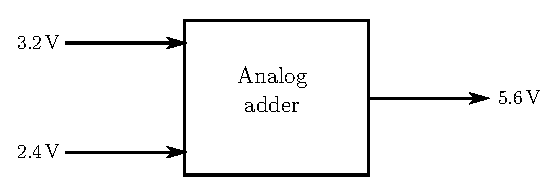
\includegraphics{chap6/addfig1.eps}
\caption{Block diagram of Analog adder}\label{fig6.1}
\end{figure}

The analog computer is constructed using linear devices like operational amplifiers. Analog computers will not be accurate because of two main reasons:
\begin{itemize}
\item[(i)] Input voltages cannot be accurately produced at all levels like 8.2\,V, 6.42\,V etc., and hence the data itself will be incorrect.

\item[(ii)] The non-linearity of the devices used to construct analog computers will not ensure stable computation over the entire range of operational voltages.
\end{itemize}

\subsection{Digital Computer}\label{sec6.1.2}

The digital computer\index{Digital computer} uses the binary number system and is constructed using gates. Only two numbers 0 and 1 are recognized by the digital computer. It overcomes the disadvantages of an analog computer as voltages corresponding to 0 and 1 can be based on threshold values, rather than on absolute values. For example any value above 2.4\,V may be considered to be at logic 1 while any value below 0.8\,V may be considered to be at logic 0.

The main disadvantage of digital computer is that more number of lines are required to represent the numbers. For example, 8 lines are need to represent 255 in decimal as 11111111 in binary. Data and instructions are represented by numbers. For example 00 could be add, 01, subtract, 10 multiply and so on. A microprocessor is a device that can perform fairly high level computation using such digital logic with binary representation of data and instructions.

\section{Decimal number system}\label{sec6.2}
\index{Decimal number system}

Number systems are fundamental in any society to quantify and represent events. The decimal number system uses the digits 0 to 9. All numbers are combination of these digits. The numbers we have in every day life like 4362, 19.217 are all compact polynomial representations.

For example the number
\begin{align}
2436.21473 &= 2000+400+30+6+0.2+0.01+0.004+0.0007+0.00003\notag\\[3pt]
           &= (2\times 1000)+(4\times 100)+(3\times 10)+(6\times 1)+(2\times 0.1)+(1\times 0.01)\notag\\[3pt]
           &\quad +(4\times 0.001)+(7\times 0.0001)+(3\times 0.00001)\notag\\[3pt]
2436.21473 &= (2\times 10^{3})+(4\times 10^{2})+(3\times 10^{1})+(6\times 10^{0})+(2\times 10^{-1})+(1\times 10^{-2})\notag\\[3pt]
&\quad +(4\times 10^{-3})+(7\times 10^{-4})+(4\times 10^{-5})\label{eq6.1}
\end{align}

Observe that the coefficient 2,4,3,6, etc., are coefficients of a polynomial in powers of 10 just like 4,6,8 and 9 are coefficients of the following polynomial in $x$:
$$
4x^{3}+6x^{2}+8x^{1}+9x^{0}
$$

The `10' in Eqn.~\eqref{eq6.1} is called the radix or base. Hence the radix or base of the decimal number system is 10. It has 10 possible numbers from 0 to 9. In general a number in a system of radix $r$ can be represented in the form of polynomial in powers of $r$ as,
\begin{align}
a_{n}a_{n-1}\ldots a_{1}a_{0}a_{-1}a_{-2}\ldots a_{-(m-1)}a_{-m} &= a_{n}r^{n}+a_{n-1}r^{n-1}+\cdots+a_{1}r^{1}+a_{0}r^{0}\notag\\[3pt]
&\quad + a_{-1}r^{-1}+\cdots+a_{-(m-1)}r^{-(m-1)}+a_{-m}r^{-m}\label{eq6.2}
\end{align}
where $a_{n}$ is the most significant digit and $a_{-m}$ is the least significant digit.

It is easy to see that Eqn.~\eqref{eq6.1} is an instance of Eqn.~\eqref{eq6.2} with
\begin{align*}
r &= 10\\[3pt]
n &= 3\\[3pt]
m &= 5
\end{align*}
and with co-efficients as
\begin{align*}
&a_{3}=2,\quad a_{2}=4,\quad a_{1}=3,\quad a_{0}=6,\quad a_{-1}=2,\quad a_{-2}=1,\\[3pt]
& a_{-3}=4,\quad a_{-4}=7,\quad \text{and}\quad a_{-5}=3
\end{align*}

\begin{example}\label{exam6.1}
Give the general polynomial representation of a number and represent decimal number 672.4935 in this representation.
\end{example}

\begin{solution}
The general polynomial representation of a number in radix $r$ number system is
$$
a_{n}r^{n}+a_{n-1}r^{n-1}+\cdots+a_{1}r^{1}+a_{0}r^{0}+a_{-1}r^{-1}+\cdots+a_{-(m-1)}r^{-(m-1)}+a_{-m}r^{-m}
$$

Now for decimal system, $r=10$ and for the given number $n=2$ and $m=4$
$$
672.4935=6\times 10^{2}+7\times 10^{1}+2\times 10^{0}+4\times 10^{-1}+9\times 10^{-2}+3\times 10^{-3}+5\times 10^{-4}
$$
\vskip -.8cm
\end{solution}

\section{Binary number system}\label{sec6.3}

From Eqn.~\eqref{eq6.2}, the general representation of a number in radix $r$ is
$$
a_{n}r^{n}+a_{n-1}r^{n-1}+\cdots+a_{1}r^{1}+a_{0}r^{0}+a_{-1}r^{-1}+\cdots+a_{-(m-1)}r^{-(m-1)}+a_{-m}r^{-m}
$$

The binary number system\index{Binary number system} has only two possible numbers 0 and 1. Hence radix $r$ is 2. The numbers 1101, 11001, 0101 and 0.11011 are examples of binary numbers and the co-efficients $a_{n}$, $a_{n-1}\ldots a_{-(m-1)}$ and $a_{-m}$ can take only one of the two possible values 0 or 1.

The binary number can be represented in polynomial form as
\begin{align}
a_{n}a_{n-1}\ldots a_{-m} &= a_{n}2^{n}+a_{n-1}2^{n-1}+\cdots+a_{1}2^{1}+a_{0}2^{0}\notag\\[3pt]
&\quad +a_{-1}2^{-1}+\cdots+a_{-(m-1)}2^{-(m-1)}+a_{-m}2^{-m}\label{eq6.3}
\end{align}

A number 1101.0101 can be represented with $n=3$ and $m=4$ as
\begin{align*}
& (1\times 2^{3})+(1\times 2^{2})+(0\times 2^{1})+(1\times 2^{0})+(0\times 2^{-1})+(1\times 2^{-2})+(0\times 2^{-3})+(1\times 2^{-4})\\[3pt]
&\hspace{5cm} =8+4+0+1+0+\dfrac{1}{4}+0+\dfrac{1}{16}\\[3pt]
&\hspace{5cm} =8+4+1+0.25+0.0625\\[3pt]
&\hspace{5cm} =13.3125\\[3pt]
&\hspace{2.4cm} \therefore \ (1101.0101)_{2}=(13.3125)_{10}
\end{align*}

The subscript indicates the radix or base of the number system to which the number in the parenthesis belongs.

\vskip .1cm

\begin{example}\label{exam6.2}
Convert the following binary number to decimal:
\begin{center}
(a)~ 1011\qquad (b)~ 110101\qquad (c)~ 10101
\end{center}
\end{example}

\begin{solution}
\begin{itemize}
\item[(a)] $(1011)_{2}=(\;?\;)_{10}$

Using the polynomial expansion of Eqn.~\eqref{eq6.3} i.e.,
$$
a_{n}2^{n}+a_{n-1}2^{n-1}+\cdots+a_{0}2^{0}+a_{-1}2^{-1}+\cdots+a_{-(m-1)}2^{-(m-1)}+a_{-m}2^{-m}
$$
with $n=3$, $a_{3}=1$, $a_{2}=0$, $a_{1}=1$, $a_{0}=1$ and all other coefficient zero becomes,
\begin{align*}
&(1\times 2^{3})+(0\times 2^{2})+(1\times 2^{1})+(1\times 2^{0})=8+2+1=1\\[3pt]
\therefore\quad &(1011)_{2}=(11)_{10} 
\end{align*}

\item[(b)] $(110101)_{2}=(\;?\;)_{10}$

Here $n=5$ and the number can be represented as
\begin{align*}
&(1\times 2^{5})+(1\times 2^{4})+(0\times 2^{3})+(1\times 2^{2})+(0\times 2^{1})+(1\times 2^{0})\\[3pt]
&= 32+16+4+1=53\\[3pt]
\therefore\quad (110101)_{2} &= (53)_{10}
\end{align*}
Notice that a two digit decimal number requires six binary bits for binary representation.

\item[(c)] $(10101)_{2}=(\;?\;)_{10}$
\begin{align*}
10101 &= (1\times 2^{4})+(0\times 2^{3})+(1\times 2^{2})+(0\times 2^{1})+(1\times 2^{0})\\[3pt]
 &= 16+4+1=21\\[3pt]
\therefore\quad (10101)_{2} &= (21)_{10}
\end{align*}
\end{itemize}
\vskip -.7cm
\end{solution}

\smallskip

\begin{example}\label{exam6.3}
Convert the following binary numbers to decimal:
\begin{center}
(a)~ $11.101$\qquad (b)~ $0.0111$\qquad (c)~ $110.1101$
\end{center}
\end{example}

\begin{solution}
\begin{itemize}
\item[(a)] $(11.101)_{2}=(\;?\;)_{10}$
\begin{align*}
11.101 &= (1\times 2^{1})+(1\times 2^{0})+(1\times 2^{-1})+(0\times 2^{-2})+(1\times 2^{-3})\\[3pt]
&= 2+1+0.5+0.125=3.625\\[3pt]
\therefore\quad (11.101)_{2} &= (3.625)_{10}
\end{align*}

\item[(b)] $(0.0111)_{2}=(\;?\;)_{10}$
\begin{align*}
0.0111 &= (0\times 2^{-1})+(1\times 2^{-2})+(1\times 2^{-3})+(1\times 2^{-4})\\[3pt]
&= 0.25+0.125+0.0625=0.4375\\[3pt]
\therefore\quad (0.0111)_{2} &= (0.4375)_{10}
\end{align*}

\item[(c)] $(110.1101)_{2}=(\;?\;)_{10}$
\begin{align*}
110.1101 &= (1\times 2^{2})+(1\times 2^{1})+(0\times 2^{0})+(1\times 2^{-1})+(1\times 2^{-2})\\[3pt]
&\quad +(0\times 2^{-3})+(1\times 2^{-4})\\[3pt]
&= 4+2+0.5+0.25+0.0625=6.8125\\[3pt]
\therefore\quad (110.1101)_{2} &= (6.8125)_{10}
\end{align*}
\end{itemize}
\vskip -.7cm
\end{solution}

\eject

\section{Decimal to binary conversion}\label{sec6.4}
\index{Decimal to binary conversion}

A typical decimal number would consist of a whole number and a fraction part like 53.4375.

The whole number part is converted to binary by repeated division by 2 in base 10 arithmetic and by keeping track of the remainder. This process is illustrated as follows:
\begin{figure}[H]
\centering
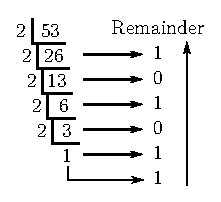
\includegraphics[scale=1.1]{chap6/fig1.eps}
\end{figure}

Read the remainder at each stage upwards as,
$$
(53)_{10}=(110101)_{2}
$$

The fraction part of the number is converted to binary by repeated multiplication of fraction part by 2 in base 10 arithmetic and by keeping track of the resulting integer as shown below until zero is encountered or until the desired number of binary places.
\begin{figure}[H]
\centering
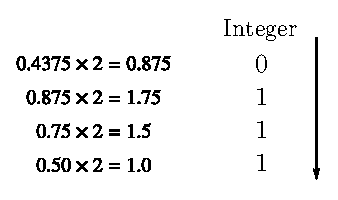
\includegraphics{chap6/fig2.eps}
\end{figure}

Read the integer at each stage downwards as
\begin{align*}
(0.4375)_{10} &= (.0111)_{2}\\[3pt]
\therefore\quad (53.4375)_{10} &= (110101.0111)_{2}
\end{align*}

\begin{example}\label{exam6.4}
Convert the following decimal numbers to binary up to four binary places.
\begin{center}
(a)~ $47.8125$\qquad (b)~ $100.0001$\qquad (c)~ $29.3749$
\end{center}
\end{example}

\eject

\begin{solution}
\begin{itemize}
\item[(a)] $(47.8125)_{10}=(\;?\;)_{2}$

Let us first convert the whole number part by repeated division by 2
\begin{figure}[H]
\centering
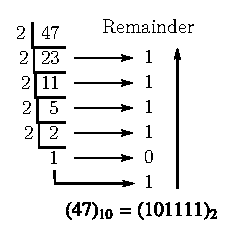
\includegraphics[scale=1.1]{chap6/fig3.eps}
\end{figure}

Now let us convert the fraction part by repeated multiplication by 2.
\begin{figure}[H]
\centering
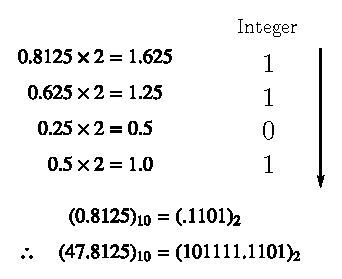
\includegraphics{chap6/fig4.eps}
\end{figure}

\item[(b)] $(100.974)_{10}=(\;?\;)_{2}$

Converting the whole number, we have
\begin{figure}[H]
\centering
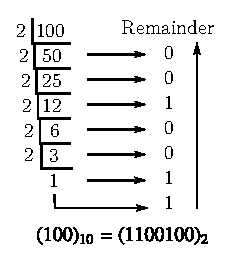
\includegraphics[scale=1.1]{chap6/fig5.eps}
\end{figure}

\eject

Now converting the fraction part, we have
\begin{figure}[H]
\centering
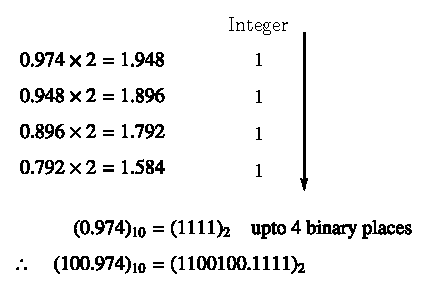
\includegraphics[scale=1.1]{chap6/fig6.eps}
\end{figure}

\item[(c)] $(29.3749)_{10}=(\;?\;)_{2}$

Converting first the whole number part, we have
\begin{figure}[H]
\centering
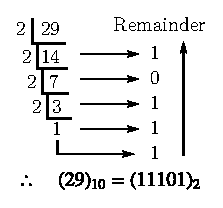
\includegraphics[scale=1.1]{chap6/fig7.eps}
\end{figure}

Next converting the fraction part we have,
\begin{figure}[H]
\centering
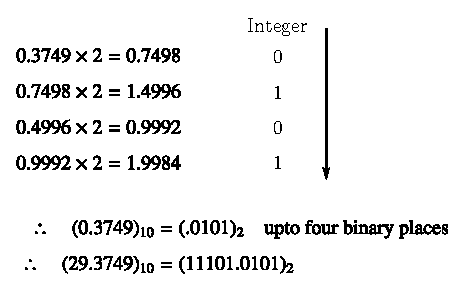
\includegraphics[scale=1.1]{chap6/fig8.eps}
\end{figure}
\end{itemize}
\vskip -.9cm
\end{solution}

\eject

\section{Octal number system with an example}\label{sec6.5}
\index{Octal number system}

From Eqn.~\eqref{eq6.2}, the general representation of a number in radix $r$ is
$$
a_{n}r^{n}+a_{n-1}r^{n-1}+\cdots+a_{1}r^{1}+a_{0}r^{0}+a_{-1}r^{-1}+\cdots+a_{-(m-1)}r^{-(m-1)}+a_{-m}r^{-m}
$$

The octal number system has 8 possible numbers from 0 to 7 and hence its radix $r=8$. The co-efficients $a_{n}$, $a_{n-1},\ldots a_{0},\ldots a_{-(m+1)}$ and $a_{-m}$ can have one of the eight possible values from 0 to 7. The octal number can be represented in polynomial form as
\begin{equation}
a_{n}a_{n-1}\ldots a_{-m}=a_{n}8^{n-1}+\cdots+a_{1}8^{1}+a_{0}8^{0}+a_{-1}8^{-1}+\cdots+a_{-(m-1)}r^{-(m-1)}+a_{-m}r^{-m}\label{eq6.4}
\end{equation}

An octal number $426.73$ can be represented as
\begin{align*}
& (4\times 8^{2})+(2\times 8^{1})+(6\times 8^{0})+(7\times 8^{-1})+(3\times 8^{-2})\\[3pt]
&= 256+16+6+0.875+0.046875\\[3pt]
&= 278.921875\\[3pt]
\therefore\quad (426.73)_{8} &= (278.921875)_{10}
\end{align*}

\begin{example}\label{exam6.5}
Convert the following octal numbers to decimal:
\begin{center}
(a)~ 243\qquad (b)~ 124.21\qquad (c)~ 0.65
\end{center}
\end{example}

\begin{solution}
\begin{itemize}
\item[(a)] $(243)_{8}=(\;?\;)_{10}$
\begin{align*}
(243)_{8} &= (2\times 8^{2})+(4\times 8^{1})+(3\times 8^{0})=128+32+3=163\\[3pt]
\therefore\quad (243)_{8} &= (163)_{10}
\end{align*}

\item[(b)]
\begin{tabbing}
$(124.21)_{8}$ \== $(1\times 8^{2})+(2\times 8^{1})+(4\times 8^{0})+(2\times 8^{-1})+(1\times 8^{-2})$\\[4pt]
\>= $64+16+4+0.25+0.015625$\\[4pt]
\>= $(84.265625)_{10}$
\end{tabbing}

\item[(c)]
\begin{tabbing}
\qquad $(0.65)_{8}$ \== $(6\times 8^{-1})+(5\times 8^{-2})$\\[4pt]
\>= $0.75+0.078125=0.828125$\\[4pt]
$\therefore$\quad~ $(0.65)_{8}$ \>= $(0.828125)_{10}$
\end{tabbing}
\end{itemize}
\vskip -.9cm
\end{solution}

\eject

\begin{example}\label{exam6.6}
Convert the following decimal numbers to octal up to 4 octal places:
\begin{center}
(a)~ 283\qquad (b)~ 847.951\qquad (c)~ 0.728
\end{center}
\end{example}

\begin{solution}
Decimal to octal conversion of whole numbers is done by repeated division by 8 and by keeping track of the remainder. The fraction part is converted by repeated multiplication by 8 and by keeping track of the integer.
\begin{itemize}
\item[(a)] $(283)_{10}=(\;?\;)_{8}$
\begin{figure}[H]
\centering
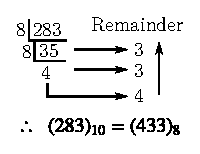
\includegraphics[scale=1.1]{chap6/fig9.eps}
\end{figure}

\item[(b)] $(847.951)_{10}=(\;?\;)_{8}$

Let us first convert the whole number part by repeated division by 8.
\begin{figure}[H]
\centering
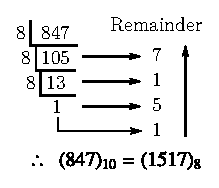
\includegraphics[scale=1.1]{chap6/fig10.eps}
\end{figure}

Next, let us convert the fraction part by repeated multiplication by 8.
\begin{figure}[H]
\centering
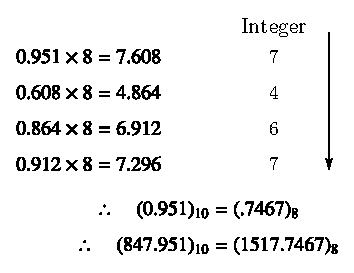
\includegraphics[scale=1.1]{chap6/fig11.eps}
\end{figure}

\eject

\item[(c)] $(0.728)_{10}=(\;?\;)_{8}$
\begin{figure}[H]
\centering
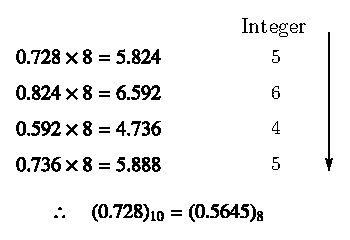
\includegraphics[scale=1.1]{chap6/fig12.eps}
\end{figure}
\end{itemize}
\vskip -.8cm
\end{solution}

\section{Table of octal-binary equivalents}\label{sec6.6}
\index{Octal-binary equivalents}

The octal-binary equivalents are shown in Table~\ref{tab6.1}.
\begin{table}[H]
\centering
\caption{Octal-binary equivalence}\label{tab6.1}
\renewcommand{\arraystretch}{1.3}
\begin{tabular}{|c|c|c|}
\hline
{\bf Octal Number} & {\bf Binary Equivalent} & {\bf Expanded Form}\\
\hline
0 & 0\,0\,0 & $0\times 2^{2}+0\times 2^{1}+0\times 2^{0}$\\[3pt]
\hline
1 & 0\,0\,1 & $0\times 2^{2}+0\times 2^{1}+1\times 2^{0}$\\[3pt]
\hline
2 & 0\,1\,0 & $0\times 2^{2}+1\times 2^{1}+0\times 2^{0}$\\[3pt]
\hline
3 & 0\,1\,1 & $0\times 2^{2}+1\times 2^{1}+1\times 2^{0}$\\[3pt]
\hline
4 & 1\,0\,0 & $1\times 2^{2}+0\times 2^{1}+0\times 2^{0}$\\[3pt]
\hline
5 & 1\,0\,1 & $1\times 2^{2}+0\times 2^{1}+1\times 2^{0}$\\[3pt]
\hline
6 & 1\,1\,0 & $1\times 2^{2}+1\times 2^{1}+0\times 2^{0}$\\[3pt]
\hline
7 & 1\,1\,1 & $1\times 2^{2}+1\times 2^{1}+1\times 2^{0}$\\[3pt]
\hline
\end{tabular}
\end{table}

\begin{example}\label{exam6.7}
Convert the following binary numbers to octal:
\begin{center}
(a)~ 1\,1\,0\,1\,1\,1\qquad (b)~ 1\,0\,1\,0\,1\,0\,1\qquad (c)~ 1\,1\,1\,0\,.\,0\,1\,1\,0\,1
\end{center}
\end{example}

\begin{solution}
For binary to octal conversion of whole numbers, group the given binary number in groups of three starting from the right most bit (least significant bit) and replace each group by the octal number shown in Table~\ref{tab6.1}.

\eject

For conversion of fraction part, make groups of three starting with the left most bit.
\begin{itemize}
\item[(a)] $(1\,1\,0\,1\,1\,1)_{2}=(\;?\;)_{8}$
\begin{figure}[H]
\centering
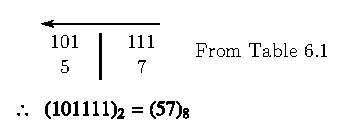
\includegraphics[scale=1.1]{chap6/fig13.eps}
\end{figure}

\item[(b)] $(1\,0\,1\,0\,1\,0\,1)_{2}=(\;?\;)_{8}$
\begin{figure}[H]
\centering
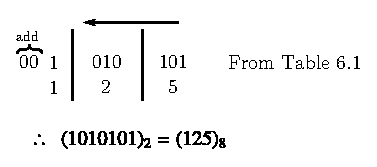
\includegraphics[scale=1.1]{chap6/fig14.eps}
\end{figure}

\item[(c)] $1\,1\,1\,0\,.\,0\,1\,1\,0\,1$

First take the whole number part
\begin{figure}[H]
\centering
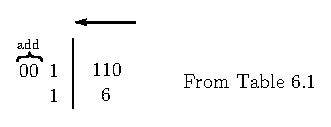
\includegraphics[scale=1.1]{chap6/fig15.eps}
\end{figure}

Next take the fraction part
\begin{figure}[H]
\centering
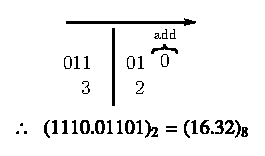
\includegraphics[scale=1.1]{chap6/fig16.eps}
\end{figure}
\end{itemize}
\vskip -.9cm
\end{solution}

\begin{example}\label{exam6.8}
Convert the following octal numbers to binary:
\begin{center}
(a)~ 724\qquad (b)~ 365.217\qquad (c)~ 0.506
\end{center}
\end{example}

\begin{solution}
To convert from octal to binary, simply replace each octal number by its binary equivalent given in Table~\ref{tab6.1}.
\begin{itemize}
\item[(a)] $(724)_{8}=(\;?\;)_{2}$

From Table~\ref{tab6.1}
$$
(724)_{8}=(111\,010\,100)_{2}
$$

\item[(b)] $(365.217)_{8}=(\;?\;)_{2}$

From Table~\ref{tab6.1}
$$
(365.217)_{8}=(011 \ 110 \ 101.010 \ 001 \ 111)_{2}
$$

\item[(c)] $(0.506)_{8}=(\;?\;)_{2}$

From Table~\ref{tab6.1}
$$
(0.506)_{8}=(0.101\,000\,110)_{2}
$$
\end{itemize}
\vskip -.9cm
\end{solution}

\section{Hexadecimal number system}\label{sec6.7}
\index{Hexadecimal number system}

The hexadecimal or hex number system has a radix of 16 with sixteen possible numbers labeled 0,1,2,3,4,5,6,7,8,9,A,B,C,D,E and F. The hexadecimal numbers with their binary and decimal equivalents are shown in Table~\ref{tab6.2}. We see from Table~\ref{tab6.2}, that each hex digit is represented by four binary bits called a {\em nibble}. We require eight bits or one byte or two nibbles to represent data and address in micro-controllers and computers, as data and address bus widths are multiples of 8 bits. From Table~\ref{tab6.2}, it is easy to see that a binary number like 10001011 can be compactly represented in hex as 8B! Thus, the hex number system provides a convenient way of representing long binary numbers. A long 32 bit binary number like
\begin{center}
\begin{tabular}{cccccccc}
1\,0\,1\,0 & 0\,1\,0\,1 & 0\,0\,1\,1 & 1\,1\,1\,0 & 1\,0\,0\,1 & 0\,1\,0\,0 & 1\,1\,1\,0 & 1\,1\,0\,0\\[3pt]
(A) & (5) & (3) & (E) & (9) & (4) & (E) & (C)
\end{tabular}
\end{center}
can be compactly represented as A53E94EC in the hexadecimal number system.

Consequently the hex number system is useful to feed instruction and data in machine language since we can enter convenient hex digits rather than long strings of binary bits.

A number in radix $r$ number system can be represented in polynomial form using Eqn.~\eqref{eq6.2} as
$$
a_{n}r^{n}+a_{n-1}r^{n-1}+\cdots+a_{1}r^{1}+a_{0}r^{0}+a_{-1}r^{-1}+\cdots+a_{-(m-1)}r^{-(m-1)}+a_{-m}r^{-m}
$$

Since the hexadecimal number system has 16 possible numbers from 0 to F, its radix is 16. The co-efficients, $a_{n},a_{n-1}\ldots a_{0}\ldots a_{m}$ can have out of the 15 possible values from 0 to F. The hexa decimal number can be represented in polynomial form as
\begin{align}
a_{n}a_{n-1}\ldots a_{-m} &= a_{n}16^{n}+a_{n-1}16^{n-1}+\cdots+a_{1}16^{1}+a_{0}16^{0}+a_{-1}16^{-1}\notag\\[3pt]
&\quad +\cdots+a_{-(m-1)}16^{-(m-1)}+a_{-m}16^{-m}\label{eq6.5}
\end{align}
\begin{table}[H]
\centering
\caption{Hexadecimal-binary-decimal equivalence}\label{tab6.2}
\index{Hexadecimal-binary-decimal equivalence}
\begin{tabular}{|c|c|c|}
\hline
{\bf Hex Number} & {\bf Binary Equivalent} & {\bf Decimal Equivalent}\\
\hline
0 & 0\,0\,0\,0 & 0\\
\hline
1 & 0\,0\,0\,1 & 1\\
\hline
2 & 0\,0\,1\,0 & 2\\
\hline
3 & 0\,0\,1\,1 & 3\\
\hline
4 & 0\,1\,0\,0 & 4\\
\hline
5 & 0\,1\,0\,1 & 5\\
\hline
6 & 0\,1\,1\,0 & 6\\
\hline
7 & 0\,1\,1\,1 & 7\\
\hline
8 & 1\,0\,0\,0 & 8\\
\hline
9 & 1\,0\,0\,1 & 9\\
\hline
A & 1\,0\,1\,0 & 10\\
\hline
B & 1\,0\,1\,1 & 11\\
\hline
C & 1\,1\,0\,0 & 12\\
\hline
D & 1\,1\,0\,1 & 13\\
\hline
E & 1\,1\,1\,0 & 14\\
\hline
F & 1\,1\,1\,1 & 15\\
\hline
\end{tabular}
\end{table}

A hexadecimal number B2D.1C can be expanded as
\begin{align*}
(B\times 16^{2})+(2\times 16^{1})+(D\times 16^{0})+(1\times 16^{-1})+(C\times 16^{-2}) &= (11\times 16^{2})+(2\times 16)\\[3pt]
&\quad +(13)+(1/16)+(12/16^{2})\\[3pt]
&= 2861.109375\\[3pt]
\therefore\quad (B2D.1C)_{16} &= (2861.109375)_{10}
\end{align*}

\noindent
{\bf Note:}
\begin{itemize}
\item From Table~\ref{tab6.1}, we find that, to represent decimal numbers from 0 to 7, we need three binary bits.

\item From Table~\ref{tab6.2}, we find that, to represent decimal numbers from 0 to 15, we need four binary bits.

\item In general

Highest Decimal number = $2^{N}-1$

$N=$ Number of binary bits.

\item For example, when $N=3$

Highest decimal number $=2^{3}-1=7$

\item As another example, when $N=4$

Highest decimal number $=2^{4}-1=15$ and so on.
\end{itemize}

\begin{example}\label{exam6.9}
Convert the following hexadecimal numbers to decimal:
\begin{center}
(a)~ FACE\qquad (b)~ 31C.DE\qquad (c)~ CAD.BF
\end{center}
\end{example}

\begin{solution}
\begin{itemize}
\item[(a)] $(FACE)_{16}=(\;?\;)_{10}$
$$
(FACE)_{16}=(F\times 16^{3})+(A\times 16^{2})+(C\times 16^{1})+(E\times 16^{0})
$$
\vskip -1.1cm
\begin{align*}
&= (15\times 16^{3})+(10\times 16^{2})+(12\times 16)+(14)\qquad\quad\\[3pt]
&= 64206\\[3pt]
\therefore~~ (FACE)_{16} &= (64206)_{10}
\end{align*}

\item[(b)] $(31C.DE)_{16}=(\;?\;)_{10}$
\begin{align*}
(31C.DE)_{16} &= (3\times 16^{2})+(1\times 16)+(12)+(13\times 16^{-1})+(14\times 16^{-2})\\[3pt]
&= 796.8671875\\[3pt]
\therefore~~ (31C.DE)_{16} &= (796.8671875)_{10}
\end{align*}

\item[(c)] $(CAD.BF)_{16}=(\;?\;)_{10}$
\begin{align*}
(CAD.BF)_{16} &= (C\times 16^{2})+(A\times 16^{1})+(D\times 16^{0})+(B\times 16^{-1})+(F\times 16^{-2})\\[3pt]
&= (12\times 16^{2})+(10\times 16)+(13)+(11\times 16^{-1})+(15\times 16^{-2})\\[3pt]
&= 3245.74609375\\[3pt]
\therefore~~ (CAD.BF)_{16} &= (3245.74609375)_{10}
\end{align*}
\end{itemize}
\vskip -.9cm
\end{solution}

\eject

\begin{example}\label{exam6.10}
Convert the following decimal numbers to hexadecimal:
\begin{center}
(a)~ 2146\qquad (b)~ 843\qquad (c)~ 2604.10546875
\end{center}
\end{example}

\begin{solution}
\begin{itemize}
\item[(a)] $(2146)_{10}=(\;?\;)_{16}$

As usual, it is done by repeated division by radix $r$ which is 16, in decimal arithmetic and by keeping tack of the remainder.
\begin{figure}[H]
\centering
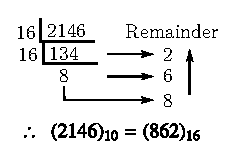
\includegraphics[scale=1.1]{chap6/fig17.eps}
\end{figure}

\item[(b)] $(843)_{10}=(\;?\;)_{16}$
\begin{figure}[H]
\centering
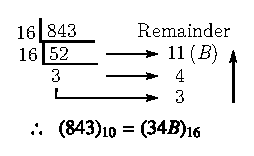
\includegraphics[scale=1.1]{chap6/fig18.eps}
\end{figure}

\item[(c)] $2604.10546875$

The whole number part is converted by repeated division by 16.
\begin{figure}[H]
\centering
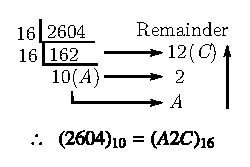
\includegraphics[scale=1.1]{chap6/fig19.eps}
\end{figure}

The fraction part is converted by repeated multiplication by 16 and by keeping track of the integer.
\begin{figure}[H]
\centering
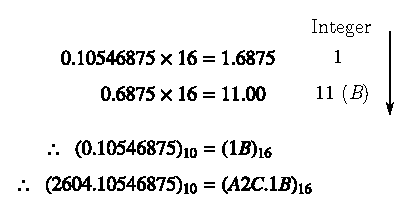
\includegraphics[scale=1.1]{chap6/fig20.eps}
\end{figure}
\end{itemize}
\vskip -1cm
\end{solution}

\medskip

\begin{example}\label{exam6.11}
Convert the following binary numbers to hexadecimal:
\begin{center}
(a)~ 1\,0\,1\,1\,1\,0\qquad (b)~ 1\,1\,0\,1\,0\,.\,1\,0\,1\qquad (c)~ 1\,0\,1\,1\,1\,0\,1\,.\,1\,1\,0\,1\,1\,1
\end{center}
\end{example}

\begin{solution}
\begin{itemize}
\item[(a)] $(101110)_{2}=(\;?\;)_{16}$

Group the whole number in groups of four bits starting from the right most bit and replace each group by the hexadecimal equivalent shown in Table~\ref{tab6.2}.

Group the fraction part in the same way starting with the left most bit.
\begin{figure}[H]
\centering
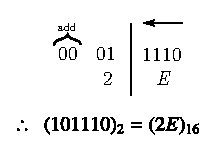
\includegraphics[scale=1.1]{chap6/fig21.eps}
\end{figure}

\item[(b)] $(11010.101)_{2}=(\;?\;)_{16}$
\begin{figure}[H]
\centering
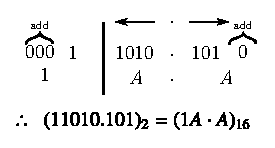
\includegraphics[scale=1.1]{chap6/fig22.eps}
\end{figure}

\item[(c)] $(1011101.110111)_{2}=(\;?\;)_{16}$
\begin{figure}[H]
\centering
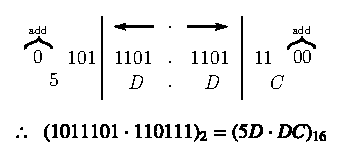
\includegraphics[scale=1.1]{chap6/fig23.eps}
\end{figure}
\end{itemize}
\vskip -1cm
\end{solution}

\eject

\section{Binary addition}\label{sec6.8}
\index{Binary addition}

Arithmetic addition of two binary numbers is similar to decimal arithmetic. Consider the addition of two decimal numbers 9 and 7.
\begin{center}
\begin{tabular}{r}
9\\
$+7$\\
\hline
16
\end{tabular}
\end{center}
which results in an answer 16 where 6 is referred to as the {\em sum} and 1 is referred to as the {\em carry}. Since binary numbers can have values of only 1 or 0, the four possible binary additions are shown in Table.~\ref{tab6.3}.
\begin{table}[H]
\centering
\caption{Binary Addition}\label{tab6.3}
\tabcolsep=1.8pt
\begin{tabular}{|cc|cc|cc|cc|}
\hline
 & Decimal & & Decimal & & Decimal & & Decimal\\
Binary & Equivalent & Binary & Equivalent & Binary & Equivalent & Binary & Equivalent\\
\hline
\begin{tabular}[t]{rr}
 & 0\\
+ & 0\\
\hline
0 & 0 \\
$\uparrow$ & $\uparrow$\\
carry & sum
\end{tabular} &
\begin{tabular}[t]{rr}
 & 0\\
+ & 0\\
\hline
& 0
\end{tabular}
&
\begin{tabular}[t]{rr}
 & 0\\
+ & 1\\
\hline
0 & 1 \\
$\uparrow$ & $\uparrow$\\
carry & sum
\end{tabular} &
\begin{tabular}[t]{rr}
 & 0\\
+ & 1\\
\hline
& 1
\end{tabular}
&
\begin{tabular}[t]{rr}
 & 1\\
+ & 0\\
\hline
0 & 1 \\
$\uparrow$ & $\uparrow$\\
carry & sum
\end{tabular} &
\begin{tabular}[t]{rr}
 & 1\\
+ & 0\\
\hline
0 & 1
\end{tabular}
&
\begin{tabular}[t]{rr}
 & 1\\
+ & 1\\
\hline
1 & 0 \\
$\uparrow$ & $\uparrow$\\
carry & sum
\end{tabular} &
\begin{tabular}[t]{rr}
 & 1\\
+ & 1\\
\hline
& 2
\end{tabular}\\
\hline
\end{tabular}
\end{table}

\begin{example}\label{exam6.12}
Add the following binary numbers:
\begin{center}
(a)~ 1\,1\,0\,1\,1~ and~ 1\,0\,1\,1\,0\qquad (b)~ 1\,1\,0\,0~ and~ 1\,1\,1\qquad (c)~ 1\,0\,.\,1\,0\,1\,1~ and~ 1\,1\,.\,0\,1\,1
\end{center}
\end{example}

\begin{solution}
\begin{itemize}
\item[(a)] $1\,1\,0\,1\,1+1\,0\,1\,1\,0$

Using Table~\ref{tab6.3}.
\begin{center}
\begin{tabular}{rr}
 & $1\,1\,0\,1\,1$\\
$+$ & $1\,0\,1\,1\,0$\\
\cline{2-2}
 & $1\,1\,0\,0\,0\,1$
\end{tabular}
\end{center}
$$
\therefore~~ 1\,1\,0\,1\,1+1\,0\,1\,1\,0=1\,1\,0\,0\,0\,1
$$

\eject

\item[(b)] $1\,1\,0\,0+1\,1\,1$
\begin{center}
\begin{tabular}{rr}
 & $1\,1\,0\,0$\\
$+$ & $0\,1\,1\,1$\\
\cline{2-2}
 & $1\,0\,0\,1\,1$
\end{tabular}
\end{center}
$$
\therefore~~ 1\,1\,0\,0+1\,1\,1=1\,0\,0\,1\,1
$$

\item[(c)] $1\,0.1\,0\,1\,1+1\,1\,.\,0\,1\,1$
\begin{center}
\begin{tabular}{rr}
 & 1\,0\,.\,1\,0\,1\,1\\
+ & 1\,1\,.\,0\,1\,1\,0\\
\cline{2-2}
 & 1\,1\,0\,.\,0\,0\,0\,1
\end{tabular}
\end{center}
$$
\therefore\quad 1\,0\,.\,1\,0\,1\,1+1\,1\,.\,0\,1\,1=1\,1\,0\,.\,0\,0\,0\,1
$$
\end{itemize}
\vskip -.9cm
\end{solution}

\section{Addition of octal numbers}\label{sec6.9}
\index{Octal number system!addition of}

Octal numbers are added just as we add decimal numbers. Convert this result to octal by division by 8 to get the sum and the carry.

This is illustrated in the following examples.
\begin{itemize}
\item[(i)] $(5)_{8}+(7)_{8}=(\;?\;)_{8}$

\medskip

\begin{tabular}{r}
5\\
$+7$\\
\hline
12
\end{tabular}

Convert decimal 12 to octal by successive division by 8 to get the sum and the carry.
\centerline{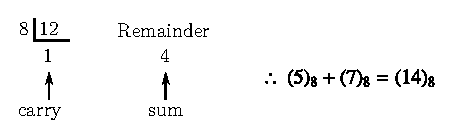
\includegraphics[scale=1.1]{chap6/fig24.eps}}

\item[(ii)] $(647)_{8}+(566)_{8}=(\;?\;)_{8}$

\medskip
\begin{tabular}{r}
647\\
$+566$\\
\hline
\end{tabular}
\end{itemize}

\begin{description}
\item[Step 1:] 
~
\begin{figure}[H]
\centering
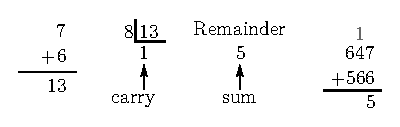
\includegraphics{chap6/fig25.eps}
\end{figure}

\item[Step 2:] 
~
\begin{figure}[H]
\centering
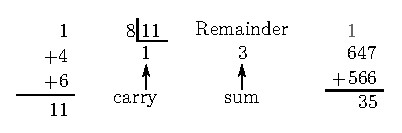
\includegraphics{chap6/fig26.eps}
\end{figure}

\item[Step 3:] 
~
\begin{figure}[H]
\centering
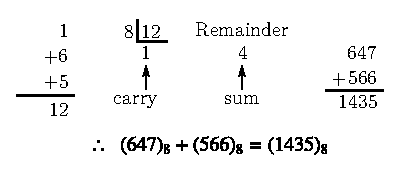
\includegraphics{chap6/fig27.eps}
\end{figure}
\end{description}

\begin{example}\label{exam6.13}
Perform addition of the following octal numbers:
\begin{center}
(a)~ $(46)_{8}$ \ and \ $(375)_{8}$\qquad (b)~ $(27.34)_{8}$ \ and \ $(11.76)_{8}$
\end{center}
\end{example}

\begin{solution}
\begin{itemize}
\item[(a)] $(46)_{8}+(375)_{8}$

\begin{tabular}{r}
46\\
+ 375\\
\hline
\end{tabular}
\begin{description}
\item[Step 1:]
~
\begin{figure}[H]
\centering
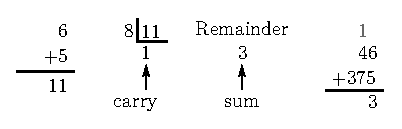
\includegraphics{chap6/fig28.eps}
\end{figure}

\eject

\item[Step 2:]
~
\begin{figure}[H]
\centering
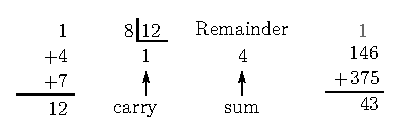
\includegraphics{chap6/fig29.eps}
\end{figure}

\item[Step 3:]
~
\begin{figure}[H]
\centering
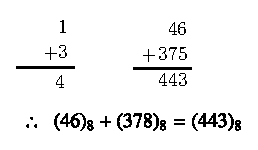
\includegraphics{chap6/fig30.eps}
\end{figure}
\end{description}

\item[(b)] $(27.34)_{8}+(11.76)_{8}$

\begin{tabular}{r}
27.34\\
+ 11.76\\
\hline
\end{tabular}
\begin{description}
\item[Step 1:]
~
\begin{figure}[H]
\centering
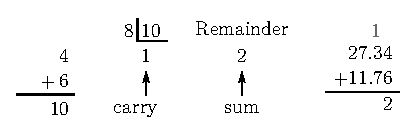
\includegraphics{chap6/fig31.eps}
\end{figure}

\item[Step 2:]
~
\begin{figure}[H]
\centering
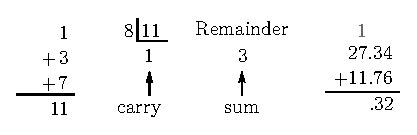
\includegraphics{chap6/fig32.eps}
\end{figure}

\item[Step 3:]
~
\begin{figure}[H]
\centering
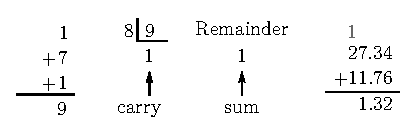
\includegraphics{chap6/fig33.eps}
\end{figure}

\eject

\item[Step 4:]
~
\begin{figure}[H]
\centering
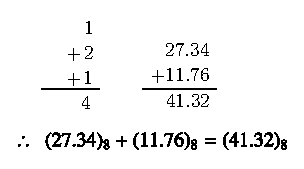
\includegraphics{chap6/fig34.eps}
\end{figure}
\end{description}
\end{itemize}
\vskip -1cm
\end{solution}

\section{Addition of hexadecimal numbers}\label{sec6.10}
\index{Hexadecimal number system!addition of}

Hexadecimal numbers are added by adding their decimal equivalents. The result is converted to hexadecimal by dividing by 16 to get the sum and the carry.

This is illustrated by the following example:
\begin{gather*}
(AB8)_{16}+(7F3)_{16}\\[4pt]
\begin{array}{r}
AB8\\
+7F3\\
\hline
\end{array}
\end{gather*}

\begin{description}
\item[Step 1:] 
~
\begin{center}
\begin{tabular}{rcl}
8 && same as decimal 8\\[3pt]
+ 3 && same as decimal 3\\
\cline{1-1} 
$11$ && $B$ in hex
\end{tabular}

\medskip

\begin{tabular}{r}
$AB8$\\
$+\;7F3$\\
\hline
$B$
\end{tabular}
\end{center}

\item[Step 2:]
~
\begin{center}
\begin{tabular}{rcr}
\begin{tabular}{r}
$B$\\
$+\;F$\\
\hline
\\
\end{tabular}
&
$\equiv$
&
\begin{tabular}{r}
$11$\\
$+\;15$\\
\hline
$26$
\end{tabular}
\end{tabular}
\end{center}

Now convert 26 to hex
\begin{figure}[H]
\centering
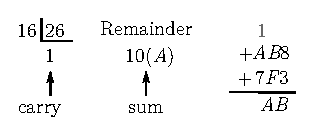
\includegraphics[scale=1.1]{chap6/fig35.eps}
\end{figure}

\item[Step 3:]
~
\begin{center}
\begin{tabular}{ccc}
\begin{tabular}{r}
\color{gray}{$1$}\\
$+\;A$\\
$+\;7$\\
\hline
\\
\end{tabular}
&
$\equiv$
&
\begin{tabular}{r}
\color{gray}{$1$}\\
$+\;10$\\
$+\;~7$\\
\hline
$18$
\end{tabular}
\end{tabular}
\end{center}

Convert 18 to hex
\begin{figure}[H]
\centering
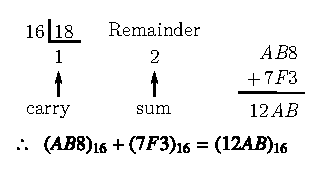
\includegraphics{chap6/fig36.eps}
\end{figure}
\end{description}

\begin{example}\label{exam6.14}
Perform addition of the following hexadecimal numbers.
\begin{itemize}
\item[(a)] $(ABC)_{16}$ \ and \ $(ABCDE)_{16}$

\item[(b)] $(DEF\cdot 12)_{16}$ \ and \ $(12EF\cdot C)_{16}$
\end{itemize}
\end{example}

\begin{solution}
\begin{itemize}
\item[(a)] $(ABC)_{16}$ \ and \ $(ABCDE)_{16}$

\smallskip
\begin{tabular}{r}
$ABC$\\
$+ABCDE$\\
\hline
\end{tabular}
\begin{description}
\item[Step 1:]
~
\begin{figure}[H]
\centering
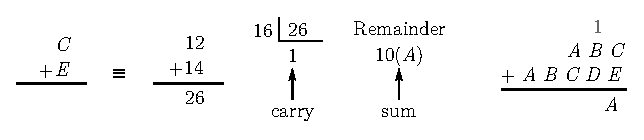
\includegraphics{chap6/fig37.eps}
\end{figure}

\item[Step 2:]
~
\begin{figure}[H]
\centering
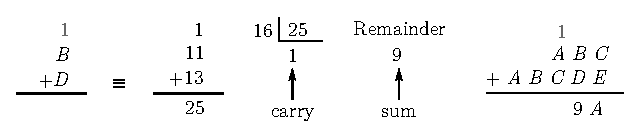
\includegraphics{chap6/fig38.eps}
\end{figure}

\item[Step 3:]
~
\begin{figure}[H]
\centering
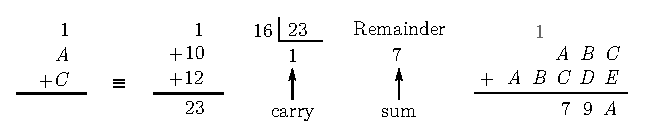
\includegraphics{chap6/fig39.eps}
\end{figure}

\item[Step 4:]
~
\begin{center}
\begin{tabular}{cccc}
\begin{tabular}{r}
$1$\\[3pt]
$+\;B$\\
\hline\\
\end{tabular}
&
$\equiv$
&
\begin{tabular}{r@{\;}l}
$1$ &\\
$+\;11$&\\
\hline
$12$ & $(C)$
\end{tabular}
&
\begin{tabular}{r}
$A~B~C$\\
$+\;A~B~C~D~E$\\
\hline
$C\,~7\,~9~~A$
\end{tabular}
\end{tabular}
\end{center}

\item[Step 5:]
~
\begin{align*}
& 
\begin{array}{r}
A~B~C\\
+\;A~B~C~D~E\\
\hline
A\,~C\,~7\,~9\,~A
\end{array}\\
\therefore\quad & (ABC)_{16}+(ABCDE)_{16}=(AC79A)_{16}
\end{align*}
\end{description}

\item[(b)] $(DEF\cdot 12)_{16}$ \ and \ $(12EF\cdot C)_{16}$

\smallskip

\begin{tabular}{r}
$DEF\cdot 12$\\[3pt]
$+12EF\cdot C0$\\
\hline
\end{tabular}

\begin{description}
\item[Step 1:]
~
\begin{center}
\begin{tabular}{cc}
\begin{tabular}{r}
2\\
$+\;0$\\
\hline
2
\end{tabular}
&
\begin{tabular}{r}
$D~E~F~\cdot~ 1~2$\\
$+\;1~2~E~F~\cdot~ C~0$\\
\hline
$2$
\end{tabular}
\end{tabular}
\end{center}

\item[Step 2:]
~
\begin{center}
\begin{tabular}{cccc}
\begin{tabular}{r}
$1$\\
$+\;C$\\
\hline\\
\end{tabular}
&
$\equiv$
&
\begin{tabular}{r@{\;}l}
$1$&\\
$+\,12$&\\
\hline
$13$ & $(D)$
\end{tabular}
&
\begin{tabular}{r}
$D~E~F~\cdot~ 1~2\,$\\
$+\;1~2~E~F~\cdot ~C~0$\\
\hline
$\cdot~\, D~2$
\end{tabular}
\end{tabular}
\end{center}

\item[Step 3:]
~
\begin{figure}[H]
\centering
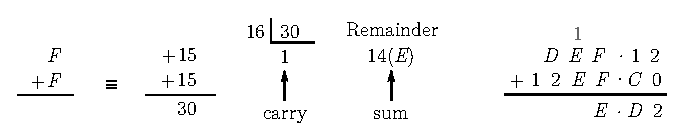
\includegraphics{chap6/fig40.eps}
\end{figure}

\item[Step 4:]
~
\begin{figure}[H]
\centering
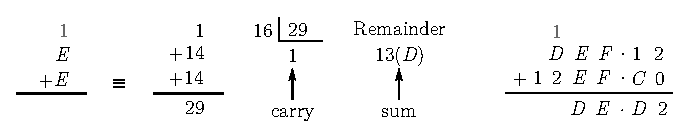
\includegraphics{chap6/fig41.eps}
\end{figure}

\item[Step 5:]
~
\begin{figure}[H]
\centering
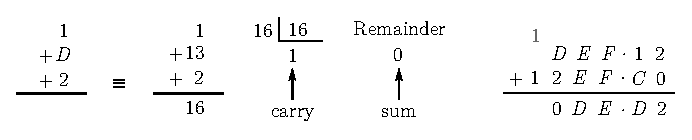
\includegraphics{chap6/fig42.eps}
\end{figure}

\item[Step 6:]
\begin{align*}
&
\begin{array}{r}
1\\
+\;1\\
\hline
2
\end{array}
\qquad\quad
\begin{array}{r}
D~E~F~\cdot~ 1\,~2\\[3pt]
+\; 1\,~2\,~E~F~\cdot ~C~0\\
\hline
2\,~0~D~E~\cdot ~D~2
\end{array}\\[7pt]
\therefore\quad & (DEF\cdot 12)_{16}+(12EF\cdot C0)_{16}=(20DE\cdot D2)_{16}
\end{align*}
\end{description}
\end{itemize}
\vskip -.9cm
\end{solution}

\section{Binary subtraction}\label{sec6.11}
\index{Binary subtraction}

Subtraction of binary numbers is similar to that of decimal numbers. When two decimal numbers are subtracted, we get a {\em difference} term and a {\em borrow} term as illustrated below:
\begin{figure}[H]
\centering
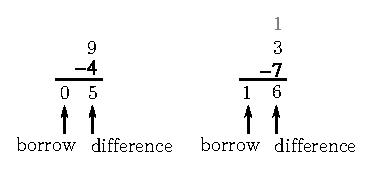
\includegraphics[scale=1.1]{chap6/fig43.eps}
\end{figure}

It is clear that, if the borrow is 0, the difference is positive and if the borrow is 1, the difference is negative.

In this case the answer is the complement of the difference. The complement of a number $n$ in radix $r$ number system is obtained by $(r-n)$, called its $r$'s complement.

Hence the 10's complement of 6 in radix 10 number system is $10-6$ or 4. Hence the result $3-7$ is $-4$.
\begin{figure}[H]
\centering
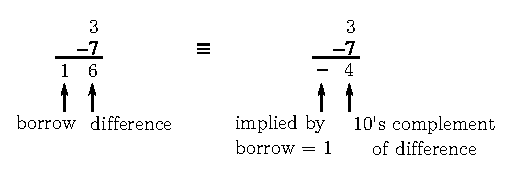
\includegraphics[scale=1.1]{chap6/fig44.eps}
\end{figure}

On similar lines the four possible binary subtractions are shown in Table \ref{tab6.4}.
\begin{table}[H]
\centering
\caption{Binary subtraction}\label{tab6.4}
\tabcolsep=1pt
\begin{tabular}{|c@{\qquad}c|c@{\qquad}c|c@{\qquad}c|c@{\qquad}c|}
\hline
{~~~\small Binary} & {\small Decimal} & {~~~\small Binary} & {\small Decimal} & {~~~\small Binary} & {\small Decimal} & {~~~\small Binary} & {\small Decimal}\\[-2pt]
       & {\small Equivalent} & & {\small Equivalent} & & {\small Equivalent} && {\small Equivalent}\\
\hline
\multicolumn{2}{|c|}{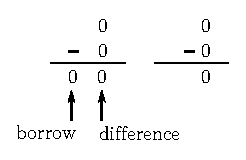
\includegraphics[scale=.9]{chap6/fig45.eps}} &
\multicolumn{2}{c|}{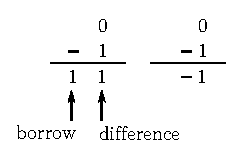
\includegraphics[scale=.9]{chap6/fig46.eps}} &
\multicolumn{2}{c|}{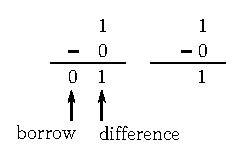
\includegraphics[scale=.9]{chap6/fig47.eps}} &
\multicolumn{2}{c|}{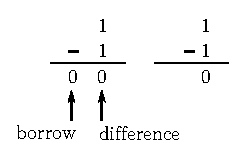
\includegraphics[scale=.9]{chap6/fig48.eps}}\\
\hline 
\end{tabular}
\end{table}

\begin{example}\label{exam6.15}
Perform the following binary subtractions.
\begin{center}
(a)~ $1011-0111$\qquad (b)~ $110.101-100.111$\qquad (c)~ $1001-1111$
\end{center}
\end{example}

\begin{solution}
\begin{itemize}
\item[(a)] $(1011)_{2}-(0111)_{2}=(\;?\;)_{2}$
\begin{figure}[H]
\centering
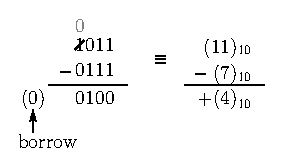
\includegraphics[scale=1.1]{chap6/fig49.eps}
\end{figure}

Zero borrow indicates that the difference is positive.
$$
\therefore\quad (1011)_{2}-(0111)_{2}=(0100)_{2}
$$

\eject

\item[(b)] $(110.101)_{2}-(100.111)=(\;?\;)_{2}$
\begin{figure}[H]
\centering
\includegraphics[scale=1.1]{chap6/fig50.eps}
\end{figure}

Once again zero borrow indicates that the difference is positive.
$$
\therefore\quad (110.101)_{2}-(100.111)_{2}=(001.110)_{2}
$$

\item[(c)] $(1001)_{2}-(111)_{2}$
\begin{figure}[H]
\centering
\includegraphics[scale=1.1]{chap6/fig51.eps}
\end{figure}

Borrow = 1 indicates that the answer is negative and the actual difference is the $r$'s complement of the difference obtained.

For the binary number system, $r=2$. The $r$'s complement or $2$'s complement can be found by adding 1 to the 1's complement. The 1's complement is found by simply inverting the bits.

For example 1's complement of 1011 is 0100 and the 2's complement of 1011 is
\begin{center}
\begin{tabular}{rl}
0~1~0~0 & ~~~ 1's complement\\
+\,1 & ~~~ +\,1\\
\cline{1-1}
0~1~0~1 & 
\end{tabular}
\end{center}

Going back to the problem, 1's complement of the difference 1010 is 0101 and the 2's complement of 1010 is
\begin{center}
\begin{tabular}{rl}
\color{gray}{1}~~ & \\
0~1~0~1 & ~~~ 1's complement\\
+\,1 & ~~~ +\,1\\
\cline{1-1}
0~1~1~0 & 
\end{tabular}
\end{center}
which is equivalent to decimal 6.

Hence $(1\,0\,0\,1)_{2}-(1\,1\,1\,1)_{2}=-(0\,1\,1\,0)_{2}$
\end{itemize}
\vskip -.9cm
\end{solution}

\begin{example}
Perform the following binary subtractions.
\begin{center}
(a)~ $1\,0\,0-1\,1\,0\,1$\qquad (b)~ $1\,0\,1\,.\,1-1\,0\,1\,1\,.\,1\,1$
\end{center}
\end{example}

\begin{solution}
\begin{itemize}
\item[(a)] $(1\,0\,0)_{2}-(1\,1\,0\,1)_{2}=(\;?\;)_{2}$
\begin{figure}[H]
\centering
\includegraphics[scale=1.1]{chap6/fig52.eps}
\end{figure}

The borrow = 1, indicates that the answer is negative and equal to the 2's complement of the difference obtained.

The 1's complement of the difference 0\,1\,1\,1 is 1\,0\,0\,0.

The 2's complement of 0\,1\,1\,1 is
\begin{center}
\begin{tabular}{r}
1\,0\,0\,0\\
+\,1\\
\hline
1\,0\,0\,1
\end{tabular}
\end{center}
which is equivalent to $(9)_{10}$.
$$
\therefore\quad (1\,0\,0)_{2}-(1\,1\,0\,1)_{2}=-(1\,0\,0\,1)_{2}
$$
\begin{figure}[H]
\centering
\includegraphics[scale=1.1]{chap6/fig53.eps}
\end{figure}

2's complement of 1\,0\,0\,1\,1\,1 is 0\,1\,1\,0\,0\,0\,+\,1 which is 0\,1\,1\,0\,0\,1
$$
\therefore\quad (1\,0\,1\,.\,1)_{2}-(1\,0\,1\,1\,.\,1\,1)_{2}=(1\,1\,0\,.\,0\,1)_{2}
$$
\end{itemize}
\vskip -.9cm
\end{solution}

\eject

\begin{example}\label{exam6.17}
Explain the method to obtain
$r$'s complement and $(r-1)$'s complement of~~ (a) decimal (b) octal (c) hexadecimal and (d) binary numbers.
\end{example}

\begin{solution}
\begin{itemize}
\item[(a)] Decimal number $(r=10)$.

Hence $r$'s complement refers to 10's complement and $(r-1)$'s complement refers to 9's compelment. The 9's complement of a single digit number $n$ is obtained as $9-n$. For example, 9's complement of 4 is $9-4=5$.

The 9's complement of a two digit number $m$ is obtained as $99-m$. For example, 9's complement of 32 is $99-32=67$. On similar lines 9's complement of a number of any size can be computed.

The 10's complement is given by,

10's complement = 9's complement $+1$
\begin{align*}
\therefore\quad \text{10's complement of 4 is } 5+1 &= 6\\[3pt]
\text{and 10's complement of 32 is } 67+1 &= 68
\end{align*}

\item[(b)] Octal number $(r=8)$.

On similar lines, the $(r-1)$'s complement or 7's complement of a single digit octal number $n$ is $7-n$.
For example, 7's complement of 6 is $7-6=1$. The 7's complement of a two digit octal number $m$ is $77-m$. For example, 7's complement of 35 is $77-35=42$. 

The 8's complement is given by
\begin{align*}
& \text{8's complement = 7's complement $+1$.}\\[3pt]
\therefore\quad & \text{8's complement of 6 is $1+1=2$, while the 8's complement of 35 is $42+1=43$.}
\end{align*}

\item[(c)] Hexadecimal number $(r=16)$

The 15's complement or $(r-1)$'s complement of a one digit hex number $n$ is $F-n$ or $15-n$ and the 15's complement of a two digit hex number $m$ is $FF-m$.

Thus the 15's complement of 6 is $F-6$ or $15-6=9$ and the 15's complement of 3 is $F-3$ or $15-3=12$ or $C$.

The 15's complement of 28 is $FF-28$. That is,
\begin{center}
\begin{tabular}{ccc}
\begin{tabular}[b]{r}
15~~~~~~\\
$-2$~~~~~~\\
\hline
$13(D)$
\end{tabular}
&
\begin{tabular}[b]{r}
15\\
$-8$\\
\hline
$7$
\end{tabular}
&
is~ D7
\end{tabular}
\end{center}

The 16's complement is given by

16's complement $=15$'s complement $+1$.

$\therefore~~ 16$'s complement of 6 is $9+1=A$

16's complement of 3 is $C+1=D$

16's complement of 28 is $D7+1=D8$

\item[(d)] Binary number $(r=2)$.

$r$'s complement refers to 2's compliment and $(r-1)$'s complement refers to 1's complement. The 1's complement of a binary number is obtained by changing 1's to 0's and 0's to 1's. The 2's complement is obtained by adding 1 to 1's complement.

i.e.,\quad 2's complement = 1's complement $+1$.

For example 1's complement of 1\,0\,0\,1 is 0\,1\,1\,0 and its 2's complement is $0~1~1~0+1=0~1~1~1$. 

\end{itemize}
Complements are useful in performing subtractions using addition operations.
\end{solution}

\begin{example}\label{exam6.18}
Perform the following decimal subtraction using (a)~$9$'s complement\break (b)~ $10$'s complement\quad (i)~ $49-24$~ (ii)~ $321-578$.
\end{example}

\begin{solution}
\begin{itemize}
\item[(i)] $49-24$
\begin{itemize}
\item[(a)] Subtraction using $9$'s complement.

Subtraction using $9$'s complement can be performed by adding the $9$'s complement of the number to be subtracted and by adding the carry to the result. When there is no carry, the result is negative and equal to the $9$'s complement of the answer.
\begin{figure}[H]
\centering
\includegraphics{chap6/fig54.eps}
\end{figure}

\eject

\item[(b)] Subtracting using $10$'s complement.

Subtraction using $10$'s complement can be perfomed by adding the $10$'s complement of the number to be subtracted and by ignoring the carry. When there is no carry, the result is negative and equal to the $10$'s complement of the answer.
\begin{figure}[H]
\centering
\includegraphics{chap6/fig55.eps}
\end{figure}
$\therefore\quad (49)_{10}-(24)_{10}=(25)_{10}$
\end{itemize}

\item[(ii)] $321-578$
\begin{itemize}
\item[(a)] Subtraction using $9$'s complement
\begin{figure}[H]
\centering
\includegraphics{chap6/fig56.eps}
\end{figure}

Hence the result is negative and equal to $9$'s complement of 742
$$
\text{i.e.,}\quad -(999-742)=-257
$$

\item[(b)] Subtraction using $10$'s complement
\begin{figure}[H]
\centering
\includegraphics{chap6/fig57.eps}
\end{figure}

Hence the result is negative and equal to $10$'s complement of 743
$$
\text{i.e.,}\quad -((999-743)+1)=-(256+1)=-257.
$$
\end{itemize}
\end{itemize}
\vskip -.85cm
\end{solution}

\begin{example}\label{exam6.19}
Perform the following binary subtractions using

\medskip

(a)~ $1$'s complement\quad (b)~ $2$'s complement

\smallskip
\qquad(i)~ $1\,0\,1\,0-1\,1\,1$\quad (ii)~ $1\,1\,0-1\,1\,0\,1$\quad (iii)~ $1\,0\cdot 0\,1\,0\,1-1\,0\,1\cdot 1\,1\,1$
\end{example}

\begin{solution}
\begin{itemize}
\item[(i)] $(1010)_{2}-(111)_{2}$
\begin{itemize}
\item[(a)] Using 1's complement
\begin{figure}[H]
\centering
\includegraphics[scale=1.1]{chap6/fig57_1.eps}
\end{figure}
\vskip -.8cm
$$
\therefore\quad (1010)_{2}-(0111)_{2}=(11)_{2}
$$

\item[(b)] Using 2's complement
\begin{figure}[H]
\centering
\includegraphics[scale=1.1]{chap6/fig57_2.eps}
\end{figure}
\end{itemize}

\eject

\item[(ii)] $(1~1~0)_{2}-(1~1~0~1)_{2}$
\begin{itemize}
\item[(a)] Using 1's complement
\begin{figure}[H]
\centering
\includegraphics[scale=1.05]{chap6/fig57_3.eps}
\end{figure}
$\therefore$\quad Answer is negative and equal to 1's complement of 1000 i.e., $-(0~1~1~1)$
$$
\therefore\quad (1~1~0)_{2}-(1~1~0~1)_{2}=-(1~1~1)_{2}
$$

\item[(b)] Using 2's complement
\begin{figure}[H]
\centering
\includegraphics[scale=1.05]{chap6/fig57_4.eps}
\end{figure}
$\therefore$\quad Answer is negative and equal to 2's complement of 1001 i.e.,
\begin{align*}
&
\begin{tabular}{l}
0~1~1~0\\[3pt]
+~~~~~~\,1\\
\hline
0~1~1~1
\end{tabular}\\[3pt]
& \therefore\quad (1~1~0)_{2}-(1~1~0~1)_{2}=-(1~1~1)_{2}
\end{align*}
\end{itemize}

\eject

\item[(iii)] $1~0~.~0~1~0~1-1~0~1~.~1~1~1$
\begin{itemize}
\item[(a)] Using 1's complement
\begin{figure}[H]
\centering
\includegraphics[scale=1.02]{chap6/fig57_5.eps}
\end{figure}
Hence answer is negative and equal to 1's complement of 
$$
1\,0\,0\,.\,0\,1\,1\,0 \quad\text{i.e.,}\quad 0\,1\,1\,.\,1\,0\,0\,1
$$
$$
\therefore\quad (1\,0\,.\,0\,1\,0\,1)_{2}-(1\,0\,1\,.\,1\,1\,1)_{2}=-(1\,1\,.\,1\,0\,0\,1)_{2}
$$

\item[(b)] Using 2's complement
\begin{figure}[H]
\centering
\includegraphics[scale=1.02]{chap6/fig57_6.eps}
\end{figure}
Ignore binary point at this stage. Hence answer is negative and equal to 2's complement of $1\,0\,0\,.\,0\,1\,1\,1$ i.e.,
\begin{align*}
& \begin{tabular}{r}
   0 1 1 . 1 0 0 0\\
               + 1\\
\hline
0 1 1 . 1 0 0 1
  \end{tabular}\\[5pt]
\therefore\quad & (1~0~.~0~1~0~1)_{2}-(1~0~1~.~1~1~1)_{2}=-(1~1~.~1~0~0~1)_{2}
\end{align*}
\end{itemize}
\end{itemize}
\vskip -.85cm
\end{solution}

\eject

\begin{example}\label{exam6.21}
Perform the following octal subtractions using (a)~ $7$'s complement (b)~ $8$'s complement\quad (i)~ $364-126$ (ii)~ $241-653$ (iii)~ $34.22-417.54$
\end{example}

\begin{solution}
\begin{itemize}
\item[(i)] $(364)_{8}-(126)_{8}=(\;?\;)_{8}$
\begin{itemize}
\item[(a)] Using $7$'s complement
\begin{figure}[H]
\centering
\includegraphics{chap6/fig61.eps}
\end{figure}
\begin{description}
\item[Step 1:] \begin{tabular}[t]{rl}
4 & \\
$+\,1$ &\\
\cline{1-1}
 5 & (a valid octal number)
\end{tabular}

\item[Step 2:] 
~

\medskip

\begin{tabular}[c]{@{\qquad}r}
\includegraphics{chap6/fig62.eps}
\end{tabular}

\item[Step 3:] 
~

\medskip

\begin{tabular}[c]{@{\qquad}r}
\includegraphics{chap6/fig62a.eps}
\end{tabular}
\end{description}

\eject

\item[(b)] Using $8$'s complement
\begin{figure}[H]
\centering
\includegraphics[scale=1.02]{chap6/fig63.eps}
\end{figure}
\begin{description}
\item[Step 1:] \begin{tabular}[t]{rl}
4 &\\
$+\,2$ & \\
\cline{1-1}
6 & (a valid octal number)
\end{tabular}

\item[Step 2:] 
~

\medskip

\begin{tabular}[c]{@{\qquad}r}
\includegraphics[scale=1.02]{chap6/fig63a.eps}
\end{tabular}

\item[Step 3:] 
~

\medskip

\begin{tabular}[c]{@{\qquad}r}
\includegraphics[scale=1.02]{chap6/fig64.eps}
\end{tabular}
\end{description}
\end{itemize}

\eject

\item[(ii)] $(241)_{8}-(653)_{8}=(\;?\;)_{8}$
\begin{itemize}
\item[(a)] Using $7$' complement
\begin{figure}[H]
\centering
\includegraphics[scale=1.05]{chap6/fig65.eps}
\end{figure}
$\therefore$~ answer is negative and equal to $7$'s complement of 365 i.e., $777-365=412$
\smallskip

$\therefore$~ $(241)_{8}-(653)_{8}=-(412)_{8}$

\item[(b)] Using $8$'s complement
\begin{figure}[H]
\centering
\includegraphics[scale=1.05]{chap6/fig66.eps}
\end{figure}
Answer is negative and equal to $8$'s complement of 366 i.e., $(777-366)+1=411+1=412$

$\therefore~ (241)_{8}-(653)_{8}=(412)_{8}$
\end{itemize}

\eject

\item[(iii)] $(34.22)_{8}-(417.54)_{8}-(\;?\;)_{8}$
\begin{itemize}
\item[(a)] Using $7$'s complement
\begin{figure}[H]
\centering
\includegraphics[scale=1.05]{chap6/fig67.eps}
\end{figure}
Hence result is negative and equal to $7$'s complement of $414.45$ i.e.,
\begin{align*}
& \begin{array}{r}
    77777\\
    -414.45\\
    \hline
    363.32
  \end{array}\\
\therefore\quad & (34.22)_{8}-(417.54)_{8}=-(363.32)_{8}
\end{align*}

\item[(b)] Using $8$'s complement
\begin{figure}[H]
\centering
\includegraphics[scale=1.05]{chap6/fig68.eps}
\end{figure}
\begin{figure}[H]
\centering
\includegraphics[scale=1.05]{chap6/fig68a.eps}
\end{figure}
Zero carry implies that the result is negative and equal to $8$'s complement of $414.46$
\begin{align*}
\text{i.e.,}\quad & (77777-41446)+1=36332\\[3pt]
\therefore\quad   & (34.22)_{8}-(417.54)_{8}=-(363.32)_{8}
\end{align*}
\end{itemize}
\end{itemize}
\vskip -.9cm
\end{solution}

\begin{example}\label{exam6.22}
Perform the following hexadecimal subtractions using (a)~ $15$'s complement (b)~ $16$'s complement.

\medskip
(i)~~ $\text{C9B4}-\text{AC4F}$\quad (ii)~ $\text{4D7}-\text{B9EA}$\quad (iii)~ $\text{B4D.A2}-\text{7C9.ED}$
\end{example}

\begin{solution}
\begin{itemize}
\item[(i)]
\begin{itemize}
\item[(a)] Using $15$'s complement
\begin{center}
\begin{tabular}{rl}
$C~9~B~4$ & $\leftarrow$ \ retain\\[3pt]
$-\,A~C~4~F$ & $\leftarrow$ \ replace by $15$'s complement\\
\cline{1-1}
\end{tabular}
\end{center}
\smallskip
$15$'s complement of $AC4F$ is $FFFF-AC4F$

$AC4F\equiv 10 \ 12 \ 4 \ 15$

$\therefore~ 15$'s complement of $AC4F$ is
\begin{align*}
& 
\begin{tabular}{rrr@{\,}lr}
15 & 15 & 15 & & 15\\
-10 & 12 & 4 & & 15\\
\hline
5 & 3 & 11 & (B) & 0
\end{tabular}\\
&
\begin{tabular}{rl}
C~9~B~4 & \\
+~5~3~B~0 & \\
\cline{1-1}
&\\[-7pt]
4 & \text{(A valid hex number)}
\end{tabular}
\end{align*}

\bigskip

\begin{description}
\item[Step 1:]
~
\vskip -.7cm

\begin{figure}[H]
\centering
\qquad\includegraphics{chap6/fig69.eps}
\end{figure}

\item[Step 2:]
~
\vskip -1.1cm

\begin{align*}
& \begin{tabular}{r}
1\\
+9\\
+3\\
\hline
13(D)
\end{tabular}\\[5pt]
&
\begin{tabular}{r}
C~9~B~4\\
+\,5~3~B~0\\
\hline
D~6~0
\end{tabular}
\end{align*}

\item[Step 3:]
~
\begin{figure}[H]
\centering
\includegraphics{chap6/fig70.eps}
\end{figure}
\end{description}

\eject

\item[(b)] Using $16$'s complements
\begin{figure}[H]
\centering
\includegraphics{chap6/fig71.eps}
\end{figure}
\end{itemize}

\item[(ii)] $(4D7)-(B9EA)_{16}=(\;?\;)_{16}$
\begin{itemize}
\item[(a)] Using $15$'s complement
\begin{align*}
&
\begin{tabular}{rl}
$04D7$ & $\leftarrow$~ retain\\
$-B9EA$ & $\leftarrow$~ replace by $15$'s complement\\
\cline{1-1}
\end{tabular}\\[5pt]
& 
\begin{tabular}{rcccc}
 & 15 & 15 & 15 & 15\\
$FFFF-B9EA\equiv$ & 11 & 9 & 14 & 10\\
\cline{2-5}
 & 4 & 6 & 1 & 5 
\end{tabular}\\
& 
\begin{tabular}{rl}
$04D7$ & \\
$+\,4615$ & (15's complement of $B9EA$)\\
\cline{1-1}
\end{tabular}
\end{align*}
\vskip -.4cm
\begin{figure}[H]
\centering
\includegraphics{chap6/fig72.eps}
\end{figure}
Zero carry indicates that the result is negative and equal to the 15's complement of $4AEC$ i.e., $FFFF-4AEC$ or
\begin{align*}
& 
\begin{tabular}{llll}
~\,15 & 15 & 15 & 15\\
$-~\,4$ & $10(A)$ & $14(E)$ & $12(C)$\\
\hline
$11(B)$ & ~5 & ~1 & ~3
\end{tabular}\\[2pt]
\therefore\quad & (4D7)_{16}-(B9EA)_{16}=-(B513)_{16} 
\end{align*}

\vfill\eject

\item[(b)] Using 16's complement
\begin{align*}
& 
\begin{tabular}{rl}
$0~4~D~7$ & $\leftarrow$~ retain\\
$-\,B~9~E~A$ & $\leftarrow$~ replace by 16's complement\\
\cline{1-1}
\end{tabular}\\[5pt]
&
\begin{tabular}{rl}
$0~4~D~7$ & \\
$+\,4~6~1~6$ & (15's complement $+1$)\\
\cline{1-1}
\end{tabular}
\end{align*}
\begin{figure}[H]
\centering
\includegraphics{chap6/fig73.eps}
\end{figure}

Zero carry indicates that the result is negative and equal to 16's complement of $4AED$ i.e., $(FFFF-4AED)+1$ or
\begin{align*}
& \begin{tabular}{lllll}
    15 & 15 & 15 & 15 & \\
     ~4 & $10(A)$ & $14(E)$ & $13(D)$ & \\
\cline{1-4}
$11(B)$ & ~5 & ~1 & ~2  \ \ +  &  $1=B513$
\end{tabular}\\[5pt]
\therefore\quad & (4D7)_{16}-(B9EA)_{16}=-(B513)_{16}
\end{align*}
\end{itemize}

\item[(iii)] $(B4D\cdot A2)_{16}-(7C9\cdot ED)_{16}$
\begin{itemize}
\item[(a)] Using 15's complement
\begin{center}
\begin{tabular}{rl}
$B4D\cdot A2$ & $\leftarrow$~ retain\\
$-7C9\cdot ED$ & $\leftarrow$~ replace by 15's complement\\
\cline{1-1}
\end{tabular}

\smallskip

\begin{tabular}{rrlrll}
 & 15 & 15 & 15 & 15 & 15\\
$FFFFF-7C9ED$ is & 7 & $12(C)$ & 9 & $14(E)$ & $13(D)$\\
\cline{2-6}
 & ~8 & ~~3 & ~6 & ~~1 & ~~2
\end{tabular}
\end{center}

{\tabcolsep=2pt
\begin{tabular}{rrrrrrr}
& $B$ & $4$ & $D$ & . & $A$ & 2\\
+ & 8 & 3 & 6 & . & 1 & 2\\
\hline
\end{tabular}}
\vskip -.5cm
\begin{figure}[H]
\centering
\includegraphics[scale=1.05]{chap6/fig74.eps}
\end{figure}

\begin{figure}[H]
\centering
\includegraphics[scale=1.05]{chap6/fig75.eps}
\end{figure}

\item[(b)] Using 16's complement
\begin{figure}[H]
\centering
\includegraphics[scale=1.05]{chap6/fig76.eps}
\end{figure}
\end{itemize}
\end{itemize}
\vskip -.85cm
\end{solution}

\section{Binary coded decimal numbers}\label{sec6.12}
\index{Binary coded decimal numbers}

Binary codes consisting of 0's and 1's are required to conveniently input data and instructions into digital systems and to interpret results. The computer performs arithmetic and logic operations on these strings of 0's and 1's. The simplest binary code is the natural binary sequence shown in Table~\ref{tab6.5}.
\begin{table}[H]
\centering
\caption{Natural binary sequence}\label{tab6.5}
\tabcolsep=12pt
\renewcommand{\arraystretch}{1.25}
\begin{tabular}{|c|cccc|}
\hline
{\bf Decimal} & \multicolumn{4}{c|}{\bf Binary Equivalent}\\
\hline
 & $b_{3}$ & $b_{2}$ & $b_{1}$ & $b_{0}$\\
\hline
0 & 0 & 0 & 0 & 0\\
1 & 0 & 0 & 0 & 1\\
2 & 0 & 0 & 1 & 0\\
3 & 0 & 0 & 1 & 1\\
4 & 0 & 1 & 0 & 0\\
5 & 0 & 1 & 0 & 1\\
6 & 0 & 1 & 1 & 0\\
7 & 0 & 1 & 1 & 1\\
8 & 1 & 0 & 0 & 0\\
9 & 1 & 0 & 0 & 1\\
10 & 1 & 0 & 1 & 0\\
11 & 1 & 0 & 1 & 1\\
12 & 1 & 1 & 0 & 0\\
13 & 1 & 1 & 0 & 1\\
14 & 1 & 1 & 1 & 0\\
15 & 1 & 1 & 1 & 1\\
\hline
\end{tabular}
\end{table}

As far as numbers are concerned, we are used to the decimal system where the first ten out of the sixteen combinations in Table~\ref{tab6.6} are sufficient to represent any decimal digit from 0 to 9. The first ten codes of the natural binary sequence is called the BCD or binary coded decimal with positional weights 8-4-2-1 as shown in Table~\ref{tab6.6}.

\eject

From Table~\ref{tab6.6}, a decimal number 437 will be represented as 
$$
(437)_{10}=(0100 \ \ 0011 \ \ 0111)_{BCD}
$$

There are only 10 valid BCD codes.

The BCD code is a 8421 code in the sense that if you add the header for locations where 1's are present, it will result in the decimal equivalent.
\begin{table}[H]
\centering
\caption{BCD representation}\label{tab6.6}
\tabcolsep=10pt
\renewcommand{\arraystretch}{1.3}
\begin{tabular}{|c|cccc|}
\hline
{\bf Decimal} & \multicolumn{4}{c|}{\bf BCD}\\
\cline{2-5}
 & 8 & 4 & 2 & 1\\
\hline
0 & 0 & 0 & 0 & 0\\
1 & 0 & 0 & 0 & 1\\
2 & 0 & 0 & 1 & 0\\
3 & 0 & 0 & 1 & 1\\
4 & 0 & 1 & 0 & 0\\
5 & 0 & 1 & 0 & 1\\
6 & 0 & 1 & 1 & 0\\
7 & 0 & 1 & 1 & 1\\
8 & 1 & 0 & 0 & 0\\
9 & 1 & 0 & 0 & 1\\
\hline
\end{tabular}
\end{table}

For example, six is represented by 0110, we have 1's under 4 and 2 in the header, giving $4+2=6$, similarly 9 is represented by 1001 with 1's under 8 and 1 in the header, giving $8+1=9$.

Note that BCD representation of decimal numbers cannot be used in arithmetic or logic operations. Can you reason out why?

\smallskip
\begin{example}\label{exam6.23}
Represent the following decimal number in BCD\quad (a)~ 821 \ (b)~ 35.67
\end{example}

\begin{solution}
\phantom{From Table~\ref{tab6.6}.}
\begin{itemize}
\item[(a)] $(821)_{10}=(1000 \ \ 0010 \ \ 0001)_{BCD}$

\item[(b)] $(35.67)_{10}=(0011 \ \ 0101 \cdot 0110 \ \ 0111)_{BCD}$
\end{itemize}
\vskip -.85cm
\end{solution}

\eject

\section{Boolean Algebra}\label{sec6.13}

Boolean Algebra\index{Boolean Algebra} is an algebra developed by George Boole\footnote[1]{George Boole ( 1815 - 1864) was an English mathematician, philosopher and logician. He worked in the fields of differential equations and algebraic logic, and is now best known as the author of The Laws of Thought.}. The laws of Boolean Algebra are used to simplify and evaluate logic expressions. Just as operations like addition (+), subtraction $(-)$, multiplication $(\times)$, and division $(\div)$ are used to evaluate arithmetic expressions, logic expressions have their own operators AND($\cdot$), OR (+) and NOT $(^{\normalfont -})$. Logic expressions evaluate to {\em true} or {\em false}. In a positive logic system true is represented by 1 while false is represented by~0.

\smallskip
\section{Logic Gates}\label{sec6.14}

A logic gate\index{Logic gate} is an electronic circuit which has one or more inputs and produces one output. The inputs to the gate are designated by the binary variables $A$, $B$, $C$ etc. and the output is denoted by the binary variable $Y$. The binary variables can take on values 0 and 1 which are electronically represented by LOW and HIGH voltage levels.

\vskip .2cm

Following are the basic logic gates.
\begin{itemize}
\item[(a)] NOT gate

\item[(b)] AND gate

\item[(c)] OR gate
\end{itemize}

\vskip .2cm

Apart from these we have some other special gates. They are:
\begin{itemize}
\item[(d)] NAND gate

\item[(e)] NOR gate

\item[(f)] Exclusive - OR (Ex-OR) gate and

\item[(g)] Exclusive - NOR (Ex-NOR) gate
\end{itemize}

\vskip .2cm

Among the gates listed above, only NOT gate has only one input. All other gates have more than one input.

\newpage

\section{The logical AND operation}\label{sec6.15}
\index{Logic gate!AND operation}

Consider the simple electric circuit shown in Fig.~\ref{fig6.2}
\begin{figure}[H]
\centering
\includegraphics{chap6/fig77_6.2.eps}
\caption{AND logic representation}\label{fig6.2}
\end{figure}

Table~\ref{tab6.7} shows the logic definition of the switch and lamp status
\begin{table}[H]
\centering
\tabcolsep=10pt
\renewcommand{\arraystretch}{1.2}
\caption{Logic definition of switch and lamp}\label{tab6.7}
\begin{tabular}{|l|c|c|}
\hline
 & {\bf\em off} & {\bf\em on}\\
\hline
Switch logic & 0 & 1\\
\hline
Lamp logic & 0 & 1\\
\hline
\end{tabular}
\end{table}

\heading{Truth Table}

Truth table lists the output of a Boolean operation for all possible combinations of the input Boolean variables.

The entire operation of the circuit can be shown in a truth-table as shown Fig.~\ref{fig6.3}.
\begin{figure}[H]
\begin{center}
\begin{minipage}[c]{2.7cm}
\begin{tabular}{|cc|c|}
\hline
{\bf A} & {\bf B} & {\bf Y}\\
\hline
0 & 0 & 0\\
0 & 1 & 0\\
1 & 0 & 0\\
1 & 1 & 1\\
\hline
\end{tabular}
\end{minipage}
\begin{minipage}[c]{6cm}
\begin{tabular}{c@{\;:\;}p{5.2cm}}
A, B & Input logic variables represented by switch position\\
Y & Output logic variable represented by lamp status
\end{tabular}
\end{minipage}
\end{center}
\caption{AND logic representation}\label{fig6.3}
\end{figure}

The first three rows say that if either one or both switches are off the lamp will be off. The logical expression is $Y=AB$.

An AND gate\index{AND gate} performs the logical AND operation and is symbolically represented as shown in Fig.~\ref{fig6.4}
\begin{figure}[H]
\centering
\includegraphics{chap6/fig78_6.4.eps}
\caption{Symbol of AND gate}\label{fig6.4}
\end{figure}

The output of a two input AND gate is at logic 1 if and only if both its inputs are at logic 1. The truth-table of the AND gate is shown in Fig.~\ref{fig6.3}. Such an AND gate can be constructed using diodes or transistors.

The logical expression for AND operation is
$$
Y=AB
$$

\section{Construction of AND gate using diodes}\label{sec6.16}

The circuit diagram of an AND gate using diodes is shown in Fig.~\ref{fig6.5}.
\begin{figure}[H]
\centering
\includegraphics{chap6/fig79_6.5.eps}
\caption{Circuit diagram of AND gate}\label{fig6.5}
\end{figure}
\begin{center}
\begin{tabular}{rlcl}
Let & $V_{1}=5V$ corresponds to $A=1$ & \Bpara{4}{-25}{0}{34} & \multirow{4}{3cm}{~~~input logic}\\[3pt]
    & $V_{1}=0V$ correspond to~\, $A=0$  & & \\[3pt]
    & $V_{2}=5V$ correspond to~\, $B=1$  & & \\[3pt]
    & $V_{2}=0V$ correspond to~\, $B=0$  & &
\end{tabular}
\end{center}
and
\begin{center}
\begin{tabular}{rcl}
$V_{o}=0V$ correspond to $Y=0$ & \Bpara{4}{-8}{0}{17} & \multirow{2}{4cm}{~~~output logic}\\[3pt]
$V_{o}=5V$ correspond to $Y=1$ & &
\end{tabular}
\end{center}

Note that $V_{1}$, $V_{2}$ and $V_{o}$ are voltages which can assume values of 0\,V and 5\,V while $A$, $B$ and $Y$ are the corresponding logic variables which can assume logic values of 0 or 1.

Let as assume that diodes are ideal with $V_{\gamma}=0$, $R_{f}=0\,\Omega$, $R_{r}=\infty$.
\begin{quote}
$V_{\gamma}=0$ implies drop across diodes = 0\,V when it conducts

$R_{f}=0$ implies diode is a short circuit when {\em on}

$R_{r}=\infty$ implies diode is an open circuit when {\em off}.
\end{quote}

When $V_{1}=0\text{\,V}$, and $V_{2}=5\text{\,V}$, cathode of $D_{1}$ is at 0\,V while its anode is at 5\,V and hence $D_{1}$ is a short circuit and $D_{2}$ is an open circuit and this situation is shown in Fig.~\ref{fig6.6}.
\begin{figure}[H]
\centering
\includegraphics{chap6/fig80_6.6.eps}
\caption{Situation when $V_{1}=0$, $V_{2}=5V$ corresponding to logic $A=0$, $B=1$}\label{fig6.6}
\end{figure}

It is easy to see that voltage at point $X$ is zero and hence $V_{o}=0V$, which corresponds to $Y=0$. The situation for all combinations of $V_{1}$ and $V_{2}$ are shown in Fig.~\ref{fig6.7}.

It is clear that the AND gate truth-table is satisfied.
\begin{center}
\tabcolsep=8pt
\renewcommand{\arraystretch}{1.2}
\begin{tabular}{|cc|c|}
\hline
{\bf A} & {\bf B} & {\bf Y}\\
\hline
0 & 0 & 0\\
0 & 1 & 0\\
1 & 0 & 0\\
1 & 1 & 1\\
\hline
\end{tabular}
\end{center}

We get the following additional information from the truth-table.
\begin{center}
\tabcolsep=8pt
\renewcommand{\arraystretch}{1.2}
\begin{tabular}{|l|}
\hline
$A\cdot 0=0$\\
$A\cdot 1=A$\\
$A\cdot A=A$\\
\hline
\end{tabular}
\end{center}
\begin{figure}[H]
\centering
\includegraphics{chap6/fig81_6.7ab.eps}

\bigskip

\includegraphics{chap6/fig81_6.7cd.eps}
\caption{Situation in AND circuit for all input combinations}\label{fig6.7}
\end{figure}

\section{The logical OR operation}\label{sec6.17}

The logical OR operation\index{Logic gate!OR operation} can be explained using the electric circuit shown in Fig.~\ref{fig6.8}.
\begin{figure}[H]
\centering
\includegraphics{chap6/fig82_6.8.eps}
\caption{Representation and truth-table of OR operation}\label{fig6.8}
\end{figure}

It is easy to see from Fig.~\ref{fig6.8}(a) that the lamp will turn {\em on} when one of the switches are {\em on}. Using the logic definition shown in Fig.~\ref{fig6.8}(b). the truth-table for OR operation can be constructed as shown in Fig.~\ref{fig6.8}(c).

An OR gate\index{OR gate} performs the logical OR operation and is symbolically represented as shown in Fig.~\ref{fig6.9}.
\begin{figure}[H]
\centering
\includegraphics{chap6/fig83_6.9.eps}
\caption{Symbol of OR gate}\label{fig6.9}
\end{figure}

The output of a two-input OR gate is at logic 1 when any one of its input or both the inputs are at logic 1.

The logical expression for OR operation is
$$
Y=A+B
$$

\eject

\section{Construction of OR gate using diodes}\label{sec6.18}

The circuit diagram of an OR gate using diodes is shown in Fig.~\ref{fig6.10}.
\begin{figure}[H]
\centering
\includegraphics{chap6/fig84_6.10.eps}
\caption{Circuit diagram of OR gate}\label{fig6.10}
\end{figure}

For the sake of analysis, we shall assume ideal diodes i.e., $V_{\gamma}=0$ and $R_{f}=0\,\Omega$ and $R_{r}=\infty$. This implies that the diode can be considered as a short circuit when {\em on} and open circuit when {\em off}.

It is easy to see that when either $V_{1}$ or $V_{2}$ or both are at 5\,V or at logic 1, the respective diodes are {\em on} (short circuit) and the voltage at point $X$ will be at 5\,V or at logic 1. When both $V_{1}$ and $V_{2}$ are at 0\,V, both $D_{1}$ and $D_{2}$ are {\em off} (open circuit) and the voltage at point $X$ is at 0\,V or at logic 0 as shown in the truth-table given in Table \ref{tab6.8}:
\begin{table}[H]
\centering
\caption{Truth-table of OR operation}\label{tab6.8}
\tabcolsep=8pt
\renewcommand{\arraystretch}{1.25}
\begin{tabular}{|cc|c|}
\hline
{\bf A} & {\bf B} & {\bf Y}\\
\hline
0 & 0 & 0\\
0 & 1 & 1\\
1 & 0 & 1\\
1 & 1 & 1\\
\hline
\end{tabular}
\end{table}

\eject

From the truth-table, we get the following additional information.
\begin{center}
\tabcolsep=8pt
\renewcommand{\arraystretch}{1.35}
\begin{tabular}{|l|}
\hline
$A+0=A$\\
$A+1=1$\\
$A+A=A$\\
\hline
\end{tabular}
\end{center}


The situations for various input combinations are shown in Fig.~\ref{fig6.11}.
\begin{figure}[H]
\centering
\includegraphics{chap6/fig85_6.11ab.eps}

\bigskip
\medskip

\includegraphics{chap6/fig85_6.11cd.eps}
\bigskip
\caption{Situations in OR circuit for all input combinations}\label{fig6.11}
\end{figure}

\section{The logical NOT operation}\label{sec6.19}

Inversion of a logic value implies a NOT operation;\index{Logic gate!NOT operation} A 1 gets inverted to 0 and a 0 to 1. If a variable,
$$
A=1,
$$
then the NOT operator acts on $A$ to invert it to 0, written as
$$
\overline{A}=0
$$

The logical symbol and the truth-table of a NOT gate\index{NOT gate} is shown in Fig.~\ref{fig6.12}.
\begin{figure}[H]
\centering
\includegraphics{chap6/fig86_6.12a.eps}
\caption{Logical symbol and Truth-table of NOT gate}\label{fig6.12}
\end{figure}

\section{Construction of NOT gate}\label{sec6.20}

The circuit diagram of a transistor based NOT gate is shown in Fig.~\ref{fig6.13}.
\begin{itemize}
\item[$\bullet$] Writing $KVL$ equation to the collector-emitter circuit, we have
$$
V_{CC}=I_{C}R_{C}+V_{CE}
$$
Also, $V_{0}=V_{CE}$

\item[$\bullet$] When $V_{i}$ is at $5V(A=1)$, the transistor is driven into saturation
\begin{gather*}
V_{CE}=V_{CC}-I_{C}R_{C}\approx 0\,V\\
\therefore\quad V_{0}=V_{CE}\approx 0\,V\\
\text{\fbox{$V_{i}=5V\ \Rightarrow \ V_{0}=0\,V$}}
\end{gather*}
\begin{figure}[H]
\centering
\includegraphics{chap6/fig87_6.13.eps}
\caption{Circuit diagram of NOT gate\index{NOR gate}}\label{fig6.13}
\end{figure}


\item[$\bullet$] When $V_{i}$ is at $0\,V (A=0)$, the transistor is off. As a result, $I_{B}=0$, $I_{C}=0$ and hence
\begin{gather*}
V_{CE}=V_{CC}=5V\\[4pt]
\therefore\quad V_{0}=V_{CE}=5V\\[4pt]
\text{\fbox{$V_{i}=0\,V\ \Rightarrow \ V_{0}=5V$}}
\end{gather*}
The truth table is shown in Fig.~\ref{fig6.14}.
\begin{figure}[H]
\centering
\begin{tabular}{ccc}
\renewcommand{\arraystretch}{1.3}
\begin{tabular}{|c|c|}
\hline
$V_{i}$ & $V_{0}$\\
\hline
$0\,V$ & $5\,V$\\[3pt]
$5\,V$ & $0\,V$\\
\hline
\end{tabular}
&
$\Rightarrow$
&
\renewcommand{\arraystretch}{1.3}
\begin{tabular}{|c|c|}
\hline
$A$ & $Y$\\
\hline
$0$ & $1$\\[3pt]
$1$ & $0$\\
\hline
\end{tabular}
\end{tabular}
\bigskip
\caption{Truth-table of NOT gate}\label{fig6.14}
\end{figure}
\end{itemize}

\eject

\section{Symbols, logic and truth-tables of the basic gates}\label{sec6.21}
\index{Logic gate!symbols}\index{Logic gate!truth-tables}

The three basic gates are: (i) AND gate\quad (ii) OR gate\quad (iii) NOT gate.

The symbol, logic and truth-table of the AND gate are shown in Fig.~\ref{fig6.15}.
\begin{figure}[H]
\centering
\includegraphics{chap6/fig89_6.15a.eps}
\caption{The AND gate}\label{fig6.15}
\end{figure}

The symbol, logic and truth-table of the OR gate are shown in Fig.~\ref{fig6.16}.
\begin{figure}[H]
\centering
\includegraphics{chap6/fig90_6.16a.eps}
\caption{The OR gate}\label{fig6.16}
\end{figure}

The symbol, logic and truth-table of the NOT gate are shown in Fig.~\ref{fig6.17}.
\begin{figure}[H]
\centering
\includegraphics{chap6/fig91_6.17a.eps}
\caption{The NOT gate}\label{fig6.17}
\end{figure}

\section{The NAND operation}\label{sec6.22}
\index{Logic gate!NAND operation}

The AND gate coupled with a NOT gate performs the NAND operation as shown in Fig.~\ref{fig6.18}.
\begin{figure}[H]
\centering
\includegraphics{chap6/fig92_6.18.eps}
\caption{The NAND gate}\label{fig6.18}
\end{figure}

The truth-table of the NAND gate\index{NAND gate} will have the $Y$ column as the inverse of that of the AND gate as shown in Fig.~\ref{fig6.19}.
\begin{figure}[H]
\centering
\tabcolsep=8pt
\renewcommand{\arraystretch}{1.2}
\begin{tabular}{|cc|c|}
\hline
{\bf A} & {\bf B} & {\bf Y}\\
\hline
0 & 0 & 1\\
0 & 1 & 1\\
1 & 0 & 1\\
1 & 1 & 0\\
\hline
\end{tabular}
\caption{Truth-table of the NAND gate}\label{fig6.19}
\end{figure}

\section{The NOR operation}\label{sec6.23}
\index{Logic gate!NOR operation}

The OR gate coupled with a NOT gate\index{NOT gate} performs the NOR operation as shown in Fig.~\ref{fig6.20}.
\begin{figure}[H]
\centering
\includegraphics{chap6/fig93_6.20.eps}
\caption{The NOR gate}\label{fig6.20}
\end{figure}

The truth-table of the NOR gate will have the $Y$ column as the inverse of that of the OR gate as shown in Fig.~\ref{fig6.21}.
\begin{figure}[H]
\centering
\tabcolsep=8pt
\renewcommand{\arraystretch}{1.25}
\begin{tabular}{|cc|c|}
\hline
{\bf A} & {\bf B} & {\bf Y}\\
\hline
0 & 0 & 1\\
0 & 1 & 0\\
1 & 0 & 0\\
1 & 1 & 0\\
\hline
\end{tabular}
\caption{Truth-table of the NOR gate}\label{fig6.21}
\end{figure}

\section{Exclusive-OR (EX-OR) gate}\label{sec6.24}
\index{Logic gate!EX-OR operation}

The EX-OR operation is defined by the boolean equation
$$
Y=A\oplus B=\overline{A}B+A\overline{B}
$$
where the operator $\oplus$ implies EX-OR operation. The logic symbol of EX-OR gate\index{EX-OR gate} is given in Fig.~\ref{fig6.22}(a) and its truth table is given in Fig.~\ref{fig6.22}(b).
\begin{figure}[H]
\centering
\includegraphics{chap6/fig94_6.22.eps}
\medskip
\caption{Logic symbol and truth table of EX-OR gate}\label{fig6.22}
\end{figure}

Observe from the truth table that, the output of EX-OR gate is high only when one input is high and the other low.

\eject

\subsection{Implementation of EX-OR gate using Basic gates}\label{sec6.24.1}

Fig.~\ref{fig6.23} shows the realisation of EX-OR gate using the basic gates.
\begin{figure}[H]
\centering
\includegraphics{chap6/fig95_6.23.eps}
\caption{EX-OR gate using basic gates}\label{fig6.23}
\end{figure}

\section{Exclusive-NOR (EX-NOR) gate}\label{sec6.25}

The EX-NOR operation\index{Logic gate!EX-NOR operation} is defined by the Boolean equation
$$
Y=A\odot B=AB+\overline{A} \ \ \overline{B}
$$
where the operator $\odot$ implies EX-NOR operation. The logic symbol of EX-NOR gate\index{EX-NOR gate} is given in Fig.~\ref{fig6.24}(a) and its truth table is given in Fig.~\ref{fig6.24}(b).
\begin{figure}[H]
\centering
\includegraphics{chap6/fig96_6.24a.eps}
\caption{Logic symbol and truth table of EX-NOR gate}\label{fig6.24}
\end{figure}
\noindent
observe from the truth table that, the output of EX-NOR gate is high only when both the inputs are same.

\subsection{Implementation of EX-NOR gate using Basic gates}\label{sec6.25.1}

Fig.~\ref{fig6.25} shows the realisation of EX-NOR gate using the basic gates
\begin{figure}[H]
\centering
\includegraphics{chap6/fig97_6.25.eps}
\caption{EX-NOR gate using Basic gates}\label{fig6.25}
\end{figure}

\section{Basic Boolean Laws}\label{sec6.26}

Following are the basic Boolean laws.\index{Boolean laws}
\begin{enumerate}
\item {\em Commutative law}
\begin{itemize}
\item[(a)] $A+B=B+A$

\item[(b)] $AB=BA$
\end{itemize}

\item {\em Associative law}
\begin{itemize}
\item[(a)] $(A+B)+C=A+(B+C)$

\item[(b)] $(AB)C=A(BC)$
\end{itemize}

\item {\em Distributive law}
\begin{itemize}
\item[(a)] $A(B+C)=AB+AC$

\item[(b)] $A+BC=(A+B)(A+C)$
\end{itemize}

\item {\em Identity law}
\begin{itemize}
\item[(a)] $A+A=A$

\item[(b)] $AA=A$
\end{itemize}

\item {\em Redundance law}
\begin{itemize}
\item[(a)] $A+AB=A$

\item[(b)] $A(A+B)=A$
\end{itemize}

\item {\em Inverse law}
\begin{itemize}
\item[(a)] $A+\overline{A}=1$

\item[(b)] $A\cdot \overline{A}=0$
\end{itemize}
\end{enumerate}

\smallskip
\begin{example}\label{exam6.24}
Prove the following Boolean laws.
\begin{itemize}
\item[(a)] $A+AB=A$

\item[(b)] $A+\overline{A}B=A+B$
\end{itemize}
\end{example}

\begin{solution}
\begin{itemize}
\item[(a)] Let us prove using the truth-table approach as shown below.
\begin{table}[H]
\centering
\caption*{Truth-table to prove $A+AB=A$}
\tabcolsep=8pt
\renewcommand{\arraystretch}{1.1}
\begin{tabular}{|cc|cc|}
\hline
\boldmath$A$ & \boldmath$B$ & \boldmath$AB$ & \boldmath$A+AB$\\
\hline
0 & 0 & 0 & 0\\
0 & 1 & 0 & 0\\
1 & 0 & 0 & 1\\
1 & 1 & 1 & 1\\
\hline
\end{tabular}
\end{table}
From the first and last columns, we observe that
$$
A+AB=A
$$
This can also be proved using the basic Boolean theorems
\begin{align*}
A+AB &= A(1+B)\\[3pt]
 &= A(1)\\[3pt]
 &= A\\[3pt]
\therefore\quad A+AB &= A
\end{align*}

\item[(b)] $A+\overline{A}B=A+B$ can be proved using the truth-table approach as shown below.
\begin{table}[H]
\centering
\caption*{Truth-table to prove $A+\overline{A}B=A+B$}
\tabcolsep=8pt
\renewcommand{\arraystretch}{1.45}
\begin{tabular}{|c|c|c|c|c|c|}
\hline
\boldmath$A$ & \boldmath$B$ & \boldmath$\overline{A}$ & \boldmath$\overline{A}B$ & \boldmath$A+\overline{A}B$ & \boldmath$A+B$\\
\hline
0 & 0 & 1 & 0 & 0 & 0\\
0 & 1 & 1 & 1 & 1 & 1\\
1 & 0 & 0 & 0 & 1 & 1\\
1 & 1 & 0 & 0 & 1 & 1\\
\hline
\end{tabular}
\end{table}
From the last two columns, we observe that
$$
A+\overline{A}B=A+B
$$
{\em Alternate method} (using basic boolean laws)
\begin{align*}
A+\overline{A}B &= A.1+\overline{A}B\\[3pt]
&= A(1+B)+\overline{A}B\quad [1+B=1]\\[3pt]
&= A+AB+\overline{A}B\\[3pt]
&= A+B[A+\overline{A}]\quad [A+\overline{A}=1]\\[3pt]
&= A+B
\end{align*}
\end{itemize}
\vskip -.95cm
\end{solution}

\begin{example}\label{exam6.25}
Prove the following Boolean identities:
\begin{itemize}
\item[(a)] $A+BC=(A+B)(A+C)$

\item[(b)] $ABC+A\overline{B}C+AB\overline{C}=AB+AC$
\end{itemize}
\end{example}

\begin{solution}
\begin{itemize}
\item[(a)] $A+BC=(A+B)(A+C)$

Let us prove this using the truth-table approach as shown below.
\begin{table}[H]
\centering
\caption*{Truth-table to prove $A+BC=(A+B)(A+C)$}
\tabcolsep=6pt
\renewcommand{\arraystretch}{1.15}
\begin{tabular}{|cccc|c|c|c|c|}
\hline
\boldmath$A$ & \boldmath$B$ & \boldmath$C$ & \boldmath$BC$ & \boldmath$A+B$ & \boldmath$A+C$ & \boldmath$A+BC$ & \boldmath$(A+B)(A+C)$\\
\hline
0 & 0 & 0 & 0 & 0 & 0 & 0 & 0\\
0 & 0 & 1 & 0 & 0 & 1 & 0 & 0\\
0 & 1 & 0 & 0 & 1 & 0 & 0 & 0\\
0 & 1 & 1 & 1 & 1 & 1 & 1 & 1\\
1 & 0 & 0 & 0 & 1 & 1 & 1 & 1\\
1 & 0 & 1 & 0 & 1 & 1 & 1 & 1\\
1 & 1 & 0 & 0 & 1 & 1 & 1 & 1\\
1 & 1 & 1 & 1 & 1 & 1 & 1 & 1\\
\hline
\end{tabular}
\end{table}

Observe from the last two columns that
$$
A+BC=(A+B)(A+C)
$$
{\em Alternate method}
\begin{align*}
\text{RHS } &= (A+B)(A+C)\\[2pt]
&= AA+AC+AB+BC\\[2pt]
&= A+AC+AB+BC\qquad [A\cdot A=A]\\[2pt]
&= A[1+C]+AB+BC\\[2pt]
&= A+AB+BC\qquad [1+C=1]\\[2pt]
&= A[1+B]+BC\\[2pt]
&= A+BC\qquad [1+B=1]\\[2pt]
&= \text{LHS}
\end{align*}

\item[(b)] $ABC+A\overline{B}C+AB\overline{C}=AB+AC$

Let us prove this using theorems of Boolean Algebra
\begin{align*}
& ABC+A\overline{B}C+AB\overline{C}\\[2pt]
&= AC(B+\overline{B})+AB\overline{C}\\[2pt]
&= AC(1)+AB\overline{C}\qquad (\text{by theorem~ } A+\overline{A}=1)\\[2pt]
&= AC+AB\overline{C}\qquad (\text{by theorem~ } A\cdot 1=1)\\[2pt]
&= A(C+\overline{C}B)\\[2pt]
&= A(C+B)\qquad (\text{By theorem~ } A+\overline{A}B=A+B)\\[2pt]
&= AB+AC
\end{align*}
\end{itemize}
\vskip -1.2cm
\end{solution}

\medskip
\begin{example}\label{exam6.26}
Construct the truth-table for the following logic expressions:
\begin{itemize}
\itemsep=0pt
\item[(a)] $f=A\overline{B}+\overline{C}$\qquad\qquad~~ 
(b)~ $f=A\overline{B}+\overline{A}B$

\item[(c)] $f=\overline{C}(\overline{B+D})$\qquad\qquad
(d)~ $f=AB+\overline{A}\overline{B}$
\end{itemize}
\end{example}

\begin{solution}
\begin{itemize}
\item[(a)] $f=A\overline{B}+\overline{C}$

The truth-table is shown in below.
\begin{table}[H]
\centering
\caption*{Truth-table to evaluate $f=A\overline{B}+\overline{C}$}
\tabcolsep=6pt
\renewcommand{\arraystretch}{1.15}
\begin{tabular}{|ccc|cccc|}
\hline
&&&&&&\\[-15pt]
\boldmath$A$ & \boldmath$B$ & \boldmath$C$ & \boldmath$\overline{B}$ & \boldmath$\overline{C}$ & \boldmath$A\overline{B}$ & \boldmath$A\overline{B}+\overline{C}$\\
\hline
0 & 0 & 0 & 1 & 1 & 0 & 1\\
0 & 0 & 1 & 1 & 0 & 0 & 0\\
0 & 1 & 0 & 0 & 1 & 0 & 1\\
0 & 1 & 1 & 0 & 0 & 0 & 0\\
1 & 0 & 0 & 1 & 1 & 1 & 1\\
1 & 0 & 1 & 1 & 0 & 1 & 1\\
1 & 1 & 0 & 0 & 1 & 0 & 1\\
1 & 1 & 1 & 0 & 0 & 0 & 0\\
\hline
\end{tabular}
\end{table}

\item[(b)] $f=A\overline{B}+\overline{A}B$

The truth-table is shown below.
\begin{table}[H]
\centering
\caption*{Truth-table to evaluate $f=A\overline{B}+\overline{C}$}
\tabcolsep=6pt
\renewcommand{\arraystretch}{1.15}
\begin{tabular}{|cc|ccccc|}
\hline
&&&&&&\\[-14pt]
\boldmath$A$ & \boldmath$B$ & \boldmath$\overline{A}$ & \boldmath$\overline{B}$ & \boldmath$A\overline{B}$ & \boldmath$\overline{A}B$ & \boldmath$A\overline{B}+\overline{A}B$\\
\hline
0 & 0 & 1 & 1 & 0 & 0 & 0\\
0 & 1 & 1 & 0 & 0 & 1 & 1\\
1 & 0 & 0 & 1 & 1 & 0 & 1\\
1 & 1 & 0 & 0 & 0 & 0 & 0\\
\hline
\end{tabular}
\end{table}
The function $f=A\overline{B}+\overline{A}B$ is the Exclusive-OR function.

\vfill\eject

\item[(c)] $f=\overline{C}(\overline{B+D})$

The truth-table is shown below.
\begin{table}[H]
\centering
\caption*{Truth-table to evaluate $f=\overline{C}(\overline{B+D})$}
\tabcolsep=6pt
\renewcommand{\arraystretch}{1.2}
\begin{tabular}{|ccc|cccc|}
\hline
&&&&&&\\[-14pt]
\boldmath$B$ & \boldmath$C$ & \boldmath$D$ & \boldmath$B+D$ & \boldmath$\overline{B+D}$ & \boldmath$\overline{C}$ & \boldmath$\overline{C}(\overline{B+D})$\\
\hline
0 & 0 & 0 & 0 & 1 & 1 & 1\\
0 & 0 & 1 & 1 & 0 & 1 & 0\\
0 & 1 & 0 & 0 & 1 & 0 & 0\\
0 & 1 & 1 & 1 & 0 & 0 & 0\\
1 & 0 & 0 & 1 & 0 & 1 & 0\\
1 & 0 & 1 & 1 & 0 & 1 & 0\\
1 & 1 & 0 & 1 & 0 & 0 & 0\\
1 & 1 & 1 & 1 & 0 & 0 & 0\\
\hline
\end{tabular}
\end{table}

\item[(d)] $f=AB+\overline{A} \ \ \overline{B}$

The truth table is shown below.
\begin{table}[H]
\centering
\tabcolsep=6pt
\renewcommand{\arraystretch}{1.15}
\begin{tabular}{|c|c|c|c|c|c|c|}
\hline
&&&&&&\\[-14pt]
\boldmath$A$ & \boldmath$B$ & \boldmath$\overline{A}$ & \boldmath$\overline{B}$ & \boldmath$AB$ & \boldmath$\overline{A} \ \ \overline{B}$ & \boldmath$AB+\overline{A} \ \ \overline{B}$\\
\hline
0 & 0 & 1 & 1 & 0 & 1 & 1\\
0 & 1 & 1 & 0 & 0 & 0 & 0\\
1 & 0 & 0 & 1 & 0 & 0 & 0\\
1 & 1 & 0 & 0 & 1 & 0 & 1\\
\hline
\end{tabular}
\end{table}
The function $f=AB+\overline{A} \ \ \overline{B}$ is the Exclusive-NOR function.
\end{itemize}
\vskip -.9cm
\end{solution}

\section{De Morgan's Theorems}\label{sec6.27}
\index{De Morgan's Theorems}\index{Logic gate!De Morgan's theorems}

De Morgan's\footnote[1]{Augustus De Morgan (27 June 1806 - 18 March 1871) was a British mathematician and logician. He formulated De Morgan's laws and introduced the term mathematical induction.} Theorems are as follows:

\begin{thm}\label{thm6.1}
The complement of a sum is equal to the product of the complements.

For two variables $A$ and $B$, this means
\begin{equation}
\overline{A+B}=\overline{A} \ \ \overline{B}\label{eq6.6}
\end{equation}
\end{thm}

\begin{thm}\label{thm6.2}
The complement of a product is equal to the sum of the complement.

For two variables $A$ and $B$, this means
\begin{equation}
\overline{AB}=\overline{A}+\overline{B}\label{eq6.7}
\end{equation}
\end{thm}

Eqns.~\eqref{eq6.6} and \eqref{eq6.7} can be easily proved using a truth-table approach as shown in Fig.~\ref{fig6.26}.
\begin{figure}[H]
\centering
\tabcolsep=6pt
\renewcommand{\arraystretch}{1.2}
\begin{tabular}{|cccccccccc|}
\hline
{\bf 1} & {\bf 2} & {\bf 3} & {\bf 4} & {\bf 5} & {\bf 6} & {\bf 7} & {\bf 8} & {\bf 9} & {\bf 10}\\
\hline
&&&&&&&&&\\[-14pt]
\boldmath$A$ & \boldmath$B$ & \boldmath$\overline{A}$ & \boldmath$\overline{B}$ & \boldmath$A+B$ & \boldmath$\overline{A+B}$ & \boldmath$\overline{A} \ \ \overline{B}$ & \boldmath$AB$ & \boldmath$\overline{AB}$ & \boldmath$\overline{A}+\overline{B}$\\
\hline
0 & 0 & 1 & 1 & 0 & 1 & 1 & 0 & 1 & 1\\
0 & 1 & 1 & 0 & 1 & 0 & 0 & 0 & 1 & 1\\
1 & 0 & 0 & 1 & 1 & 0 & 0 & 0 & 1 & 1\\
1 & 1 & 0 & 0 & 1 & 0 & 0 & 1 & 0 & 0\\
\hline
\end{tabular}
\caption{Truth-table to prove De Morgan's Theorems}\label{fig6.26}
\end{figure}

Observe that columns 6 and 7 prove Theorem~\ref{thm6.1} while columns 9 and 10 prove Theorem~\ref{thm6.2}. De Morgan's Theorem is useful in the simplification of complemented Boolean expressions.

\section{Universal gates}\label{sec6.28}
\index{Universal gates}

NAND and NOR gates are called universal\index{Logic gate!universal} logic gates, since any logic operation can be realised using these gates.

\begin{example}\label{exam6.27}
Realise the following gates using NAND gates.
\begin{center}
\begin{tabular}{r@{\;\,}l@{\qquad}r@{\;\,}l@{\qquad}r@{\;\,}l}
(a) & NOT gate & (b) & AND gate & (c) & OR gate\\[4pt]
(d) & NOR gate & (e) & EX-OR gate & (f) & EX-NOR gate
\end{tabular}
\end{center}
\end{example}

\begin{solution}
\begin{itemize}
\item[(a)] {\bf NOT gate using NAND}\index{NOT gate!using NAND}

The NOT logic is
\begin{align*}
Y &= \overline{A}\\[3pt]
&= \overline{A\cdot A}
\end{align*}

\eject

The NOT gate using NAND gate is shown below.
\begin{figure}[H]
\centering
\includegraphics{chap6/fig98.eps}
\end{figure}

\item[(b)] {\bf AND gate using NAND}\index{AND gate!using NAND}

The AND logic is
\begin{align*}
Y &= AB\\[3pt]
  &= \overline{\overline{AB}}
\end{align*}

Observe that, the AND operation is obtained by NAND followed NOT operation. The AND gate using NAND gates is shown below.
\begin{figure}[H]
\centering
\includegraphics{chap6/fig99.eps}
\end{figure}

\item[(c)] {\bf OR gate using NAND}\index{OR gate!using NAND}

The OR logic is
\begin{align*}
Y &= A+B\\[3pt]
&= \overline{\overline{A+B}}\\[3pt]
&= \overline{\overline{A}\cdot \overline{B}}
\end{align*}

The OR gate using NAND gates is shown below.
\begin{figure}[H]
\centering
\includegraphics{chap6/fig100.eps}
\end{figure}

\item[(d)] {\bf NOR gate using NAND}\index{NOR gate!using NAND}

To obtain NOR gate, we have to put one NOT gate at the output of OR gate obtained in part (c), as shown below.
\begin{figure}[H]
\centering
\includegraphics{chap6/fig101.eps}
\end{figure}

\item[(e)] {\bf EX-OR gate using NAND}\index{EX-OR gate!using NAND}

The EX-OR logic is
$$
Y=\overline{A}B+A\overline{B}
$$
Complementing twice, we have
\begin{align*}
Y &= \overline{\overline{\overline{A}B+A\overline{B}}}\\[3pt]
  &= \overline{\overline{\overline{A}B}\cdot \overline{A\overline{B}}}
\end{align*}

The EX-OR gate using NAND gates is shown below.
\begin{figure}[H]
\centering
\includegraphics{chap6/fig102.eps}
\end{figure}

\eject

\item[(f)] {\bf EX-NOR gate using NAND}\index{EX-NOR gate!using NAND}

The EX-NOR logic is
\begin{align*}
Y &= AB+\overline{A} \ \ \overline{B}\\[3pt]
&= \overline{\overline{AB+\overline{A} \ \ \overline{B}}}\qquad \text{(complementing twice)}\\[3pt]
&= \overline{\overline{AB}\cdot \overline{\overline{A} \ \ \overline{B}}}
\end{align*}

The EX-NOR gate using NAND gates is shown below.
\begin{figure}[H]
\centering
\includegraphics{chap6/fig103.eps}
\end{figure}
\end{itemize}
\end{solution}

\begin{example}\label{exam6.28}
Realise the following gates using NOR gates.
\begin{center}
\begin{tabular}{r@{\;\,}l@{\qquad}r@{\;\,}l@{\qquad}r@{\;\,}l}
(a) & NOT gate & (b) & AND gate & (c) & OR gate\\[3pt]
(d) & NAND gate & (e) & EX-OR gate & (f) & EX-NOR gate 
\end{tabular}
\end{center}
\end{example}

\begin{solution}
\begin{itemize}
\item[(a)] {\bf NOT gate using NOR}\index{NOT gate!using NOR}

The NOT logic is
$$
Y=\overline{A}=\overline{A+A}
$$

\eject

The NOT gate using NOR gate is shown below.
\begin{figure}[H]
\centering
\includegraphics{chap6/fig104.eps}
\end{figure}

\item[(b)] {\bf AND gate using NOR}\index{AND gate!using NOR}

The AND logic is
\begin{align*}
Y &= AB\\[3pt]
&= \overline{\overline{AB}}\qquad \text{(complementing twice)}\\[3pt]
&= \overline{\overline{A}+\overline{B}}
\end{align*}
The AND gate using NOR gates is shown below.
\begin{figure}[H]
\centering
\includegraphics{chap6/fig105.eps}
\end{figure}

\item[(c)] {\bf OR gate using NOR}\index{OR gate!using NOR}

The OR logic is
\begin{align*}
Y &= A+B\\[3pt]
&= \overline{\overline{A+B}}\qquad \text{(complementing twice)}
\end{align*}
The OR gate using NOR gates is shown below.
\begin{figure}[H]
\centering
\includegraphics{chap6/fig106.eps}
\end{figure}

\item[(d)] {\bf NAND gate using NOR}\index{NAND gate!using NOR}

To obtain NAND gate, we have to put one NOT gate at the output of AND gate obtained in part (b) as shown below.
\begin{figure}[H]
\centering
\includegraphics{chap6/fig107.eps}
\end{figure}

\item[(e)] {\bf EX-OR gate using NOR}\index{EX-OR gate!using NOR}

To implement EX-OR gate using only NOR gates we need to get the
expression for $\overline{Y}$. This can be done by using the
truth-table of EX-OR gate, which is shown below. 
\begin{center}
\renewcommand{\arraystretch}{1.2}
\tabcolsep=8pt
\begin{tabular}{|c|c|c|c|}
\hline
$A$ & $B$ & $Y$ & $\overline{Y}$\\
\hline
0 & 0 & 0 & 1\\
0 & 1 & 1 & 0\\
1 & 0 & 1 & 0\\
1 & 1 & 0 & 1\\
\hline
\end{tabular}
\end{center}

From the truth table we find that, $\overline{Y}=1$ for
$A=B=0(\overline{A}=\overline{B}=1)$ or $A=B=1$.
\begin{align*}
\text{i.e.,}\qquad \overline{Y} &= \overline{A}
\ \ \overline{B}\quad\text{or}\quad AB\\[3pt]
\overline{Y} &= \overline{A} \ \ \overline{B}+AB\quad\text{[Replacing
    or by logical OR symbol]}
\end{align*}
Applying De Morgan's theorem to each term on the RHS, we have
\begin{align*}
\overline{Y} &= \overline{\overline{\overline{A}
    \ \ \overline{B}}}+\overline{\overline{A B}}\quad
\text{(complementing each term twice)}\\[3pt]
\overline{Y} &= \overline{A+B}+\overline{\overline{A}+\overline{B}}
\end{align*}
Complementing both sides,
$$
Y=\overline{\overline{A+B}+\overline{\overline{A}+\overline{B}}}
$$

\eject

The EX-OR gate using NOR gates is shown below.
\begin{figure}[H]
\centering
\includegraphics{chap6/fig108.eps}
\end{figure}

\item[(f)] {\bf EX-NOR gate using NOR}\index{EX-NOR gate!using NOR}

To implement EX-NOR gate using only NOR gates we need to get the
expression for $\overline{Y}$. This can be done by using the truth
table of EX-NOR gate, which is shown below.
\begin{center}
\renewcommand{\arraystretch}{1.2}
\tabcolsep=8pt
\begin{tabular}{|c|c|c|c|}
\hline
$A$ & $B$ & $Y$ & $\overline{Y}$\\
\hline
0 & 0 & 1 & 0\\
0 & 1 & 0 & 1\\
1 & 0 & 0 & 1\\
1 & 1 & 1 & 0\\
\hline
\end{tabular}
\end{center}

From the truth table we find that, $\overline{Y}=1$ for $A=0$ and
$B=1$ ($\overline{A}=1$ and $B=1$) or $A=1$ and $B=0$ ($A=1$ and
$\overline{B}=1$).
\begin{align*}
\text{i.e.,}\quad \overline{Y} &= \overline{A}B\quad\text{or}\quad
A\overline{B}\\[3pt]
\overline{Y} &= \overline{A}B+A\overline{B}\quad \text{[Replacing or
    by logical OR symbol]} 
\end{align*}
Applying De Morgan's theorem to each term on the RHS, we have
\begin{align*}
\overline{Y}
&=\overline{\overline{\overline{A}B}}+\overline{\overline{A\overline{B}}}\\[3pt]
\overline{Y} &= \overline{A+\overline{B}}+\overline{\overline{A}+B}
\end{align*}
complementing both sides,
$$
Y=\overline{\overline{A+\overline{B}}+\overline{\overline{A}+B}}
$$
The EX-NOR gate using NOR gates is shown below.
\begin{figure}[H]
\centering
\includegraphics{chap6/fig109.eps}
\end{figure}
\end{itemize}
\vskip -1cm
\end{solution}

\smallskip
\begin{example}\label{exam6.29}
Simplify and realize the following Boolean expressions using logic gates.
\begin{itemize}
\item[(a)] $Y=\overline{\overline{BC}+\overline{AD}(\overline{AB}+\overline{CD})}$

\item[(b)] $Y=(A+B\overline{C})(\overline{A}+B+\overline{C})$
\end{itemize}
\end{example}

\begin{solution}
\begin{itemize}
\item[(a)]
Applying De Morgan's Theorem to the RHS, treating $x=\overline{BC}$
and $y=\overline{AD}(\overline{AB}+\overline{CD})$ we have,
\begin{align*}
\text{RHS}=\overline{x+y} &= \overline{x}\cdot \overline{y}\\[2pt]
\therefore\quad Y &= (\overline{\overline{BC}})(\overline{\overline{AD}(\overline{AB}+\overline{CD})})\\[2pt]
&= BC(\overline{\overline{AD}(\overline{AB}+\overline{CD})})
\end{align*}
Applying De Morgan's Theorem to $(\overline{\overline{AD}(\overline{AB}+\overline{CD})})$ treating $x=\overline{AD}$ and $y=\overline{AB}+\overline{CD}$, we have
\begin{align*}
Y &= BC(\overline{\overline{AD}}+\overline{\overline{AB}+\overline{CD}})\\
  &= BC(AD+\overline{\overline{AB}+\overline{CD}})
\end{align*}
Now applying De Morgan's Theorem to $\overline{\overline{AB}+\overline{CD}}$ we have
\begin{align*}
Y &= BC(AD+\overline{\overline{AB}}\cdot \overline{\overline{CD}})\\
&= BC(AD+ABCD)\\
&= ABCD+ABCD\\[3pt]
\therefore\quad Y &= ABCD
\end{align*}
This can be implemented using a four input AND gate as shown below.
\begin{figure}[H]
\centering
\includegraphics{chap6/fig110.eps}
\caption*{Implementation of $Y=ABCD$}
\end{figure}

\item[(b)] $Y=(A+B\overline{C})(\overline{A}+B+\overline{C})$. Using the Basic Boolean Theorem, we have,
\begin{align*}
Y &= (A\overline{A}+AB+A\overline{C}+\overline{A}B\overline{C}+B\overline{C}+B\overline{C})\\[3pt]
&= (AB+A\overline{C}+\overline{A}B\overline{C}+B\overline{C})\\[3pt]
&= AB+A\overline{C}+B\overline{C}(\overline{A}+1)\\[3pt]
&= AB+A\overline{C}+B\overline{C}\\[3pt]
Y &= AB+\overline{C}(A+B)
\end{align*}
The implementation of the expression is shown below.
\begin{figure}[H]
\centering
\includegraphics{chap6/fig111.eps}
\caption*{Implementation of $Y=AB+\overline{C}(A+B)$}
\end{figure}
\end{itemize}
\vskip -1.2cm
\end{solution}

\eject

\begin{example}\label{exam6.30}
Simplify and implement the following Boolean expression using logic gates:
\begin{itemize}
\item[(a)] $Y=AB+\overline{A}C+BC$

\item[(b)] $Y=(A+\overline{B}+\overline{C})(A+\overline{B}+C)$

\item[(c)] $Y=C(B+C)(A+B+C)$
\end{itemize}
\end{example}

\smallskip
\begin{solution}
\begin{itemize}
\item[(a)] $Y=AB+\overline{A}C+BC$

$A+\overline{A}=1$. Hence multiplication of the term $BC$ by $(A+\overline{A})$ does not alter the logic.
\begin{align*}
Y &= AB+\overline{A}C+BC(A+\overline{A})\\[6pt]
  &= AB+\overline{A}C+ABC+\overline{A}BC\\[6pt]
  &= AB+ABC+\overline{A}C+\overline{A}BC\\[6pt]
  &= AB(1+C)+\overline{A}C(1+B)\\[6pt]
Y &= AB+\overline{A}C
\end{align*}
The implementation is shown below.
\begin{figure}[H]
\centering
\includegraphics{chap6/fig112.eps}
\caption*{Implementation of $Y=AB+\overline{A}C$}
\end{figure}

\eject

\item[(b)] $Y=(A+\overline{B}+\overline{C})(A+\overline{B}+C)$

\vskip .15cm
Multiplying out the terms on the RHS, we have
\begin{align*}
Y &= AA+A\overline{B}+AC+A\overline{B}+\overline{B}
\ \ \overline{B}+\overline{B}C+A\overline{C}+\overline{B} \ \ \overline{C}+\overline{C}C\\[5pt]
&=
A+A\overline{B}+AC+\overline{B}+\overline{B}C+A\overline{C}+\overline{B}
\ \ \overline{C}\\[5pt]
&= A(1+\overline{B})+AC+\overline{B}(1+C)+A\overline{C}+\overline{B}
\ \ \overline{C}\\[5pt]
&= A+AC+\overline{B}+\overline{B} \ \ \overline{C}+A\overline{C}\\[5pt]
&= A(1+C)+\overline{B}(1+\overline{C})+A\overline{C}\\[5pt]
&= A+\overline{B}+A\overline{C}\\[5pt]
&= A(1+\overline{C})+\overline{B}\\[5pt]
Y &= A+\overline{B}
\end{align*}
The implementation is shown below.
\begin{figure}[H]
\centering
\includegraphics{chap6/fig113.eps}
\caption*{Implementation of $Y=A+\overline{B}$}
\end{figure}

\item[(c)] $Y=C(B+C)(A+B+C)$

One way of simplification is by multiplying the terms out and by applying the laws of Boolean algebra. A more elegant way of simplification is to repeatedly apply De Morgan's Theorem.

Taking the complement of both LHS and RHS, we have
$$
\overline{Y}=\overline{C(B+C)(A+B+C)}
$$

\eject
\noindent
Applying De Morgan's Theorem to the RHS, we have
$$
\overline{Y}=\overline{C}+(\overline{B+C})+(\overline{A+B+C})
$$
Applying De Morgan's Theorem to the $2^{\text{nd}}$ and $3^{\text{rd}}$ terms on the RHS, we have,
\begin{align*}
\overline{Y} &= \overline{C}+\overline{B}
\ \ \overline{C}+\overline{A} \ \ \overline{B} \ \ \overline{C}\\[4pt]
&= \overline{C}+\overline{B} \ \ \overline{C}(1+\overline{A})\\[4pt]
&= \overline{C}+\overline{B} \ \ \overline{C}\\[4pt]
&= \overline{C}(1+\overline{B})\\[4pt]
\overline{Y} &= \overline{C}\qquad \text{or}\qquad Y = C
\end{align*}
The implementation is shown below.
\begin{figure}[H]
\centering
\includegraphics{chap6/fig113a.eps}
\caption*{Implementation of $Y=C$}
\end{figure}
\end{itemize}
\vskip -1cm
\end{solution}

\smallskip
\begin{example}\label{exam6.31}
Simplify the following expressions and implement using NAND gates only
\begin{itemize}
\item[(a)] $XYZ+YZ+\overline{Z}$

\item[(b)] $(A+\overline{B}C)(\overline{A}+B+\overline{C})(A+\overline{B})$
\end{itemize}
\end{example}

\begin{solution}
\begin{itemize}
\item[(a)] $XYZ+YZ+\overline{Z}$

Let the function be
\begin{align*}
F &= XYZ+YZ+\overline{Z}\\[5pt]
  &= YZ(X+1)+\overline{Z}\\[5pt]
  &= YZ+\overline{Z}
\end{align*}
$\therefore$~ $F=\overline{Z}+ZY$.

\eject

$\overline{Z}+ZY$ is of the form $A+\overline{A}B$.
\begin{align*}
\text{But}\qquad A+\overline{A}B &=A+B\\[4pt]
\text{with}\qquad A &=\overline{Z}\quad\text{and}\quad B=Y\\[4pt]
\overline{Z}+ZY &=\overline{Z}+Y\\[4pt]
\therefore\quad F &= \overline{Z}+Y
\end{align*}
To implement using only NAND gates, we need a complemented product term.

Complementing both LHS and RHS, we have
\begin{align*}
\overline{F} &= \overline{\overline{Z}+Y}\\[4pt]
             &= \overline{\overline{Z}}\cdot \overline{Y}\\[4pt]
\overline{F} &= Z\overline{Y}
\end{align*}
Complementing both LHS and RHS again, we have
$$
F=\overline{Z\overline{Y}}
$$
This can be implemented using only NAND gate as shown below.
\begin{figure}[H]
\centering
\includegraphics{chap6/fig114.eps}
\caption*{NAND Implementation of $F=\overline{Z}+Y$}
\end{figure}

\item[(b)] Let $F=(A+\overline{B}C)(\overline{A}+B+\overline{C})(A+\overline{B})$.

Multiplying out the RHS, we have
\begin{align*}
F &= (AB+A\overline{C}+\overline{A} \ \ \overline{B}C)(A+\overline{B})\\[4pt]
&= AB+A\overline{C}+A\overline{B} \ \ \overline{C}+\overline{A} \ \ \overline{B}C\\[4pt]
&= AB+A\overline{C}(1+\overline{B})+\overline{A} \ \ \overline{B}C\\[5pt]
F &= AB+A\overline{C}+\overline{A} \ \ \overline{B} \ \ C
\end{align*}
Complementing both sides, we have
$$
\overline{F}=\overline{AB+A\overline{C}+\overline{A} \ \ \overline{B}C}
$$
Applying De Morgan's Theorem to RHS we have
$$
\overline{F}=\overline{AB}\cdot \overline{A\overline{C}}\cdot
\overline{\overline{A} \ \ \overline{B}C}
$$
Complementing both sides once again, we have
$$
F=\overline{\overline{AB}\cdot \overline{A\overline{C}}\cdot
  \overline{\overline{A} \ \ \overline{B}C}}
$$
The implementation of this expression using only NAND gates is shown below.
\begin{figure}[H]
\centering
\includegraphics{chap6/fig115.eps}
\caption*{NAND Implementation of $F=AB+A\overline{C}+\overline{A} \ \ \overline{B}C$}
\end{figure}
\end{itemize}
\vskip -.9cm
\end{solution}

\eject

\begin{example}\label{exam6.32}
Simplify and implement the following expressions using only NOR gates.
\begin{itemize}
\item[(a)] $Y=\overline{(A+\overline{B}+C)(\overline{A}+B+C)(A+B)}$

\item[(b)] $Y=(A+B)(A+\overline{B})(\overline{A}+B)$

\item[(c)] $Y=\overline{A}BC+A\overline{B}C+ABC$
\end{itemize}
\end{example}

\smallskip
\begin{solution}
\begin{itemize}
\item[(a)] $Y=\overline{(A+\overline{B}+C)(\overline{A}+B+C)(A+B)}$

\vskip .1cm
Complementing both sides,
$$
\overline{Y}=(A+\overline{B}+C)(\overline{A}+B+C)(A+B)
$$
Multiply out the RHS, we have
\begin{align*}
\overline{Y} &= (AB+AC+\overline{A} \ \ \overline{B}+\overline{B}C+\overline{A}C+BC+C)(A+B)\\[4pt]
\text{Now}\qquad BC+C &= C(1+B)=C\\[4pt]
\therefore\quad \overline{Y} &= (AB+AC+\overline{A}
\ \ \overline{B}+\overline{B} \ \ C+\overline{A}C+C)(A+B)\\[4pt]
&= AB+AB+AC+ABC+A\overline{B}C+\overline{A}BC+AC+BC\\[4pt]
&=AB+AC+ABC+A\overline{B}C+\overline{A}BC+AC+BC\\[4pt]
&=AB+ABC+AC+A\overline{B}C+\overline{A}BC+BC\\[4pt]
&= AB(1+C)+AC(1+\overline{B})+BC(1+\overline{A})\\[4pt]
\therefore\quad \overline{Y} &= AB+AC+BC
\end{align*}
Applying De Morgan's Theorem to each term on the RHS,
$$
\overline{Y}=(\overline{\overline{A}+\overline{B}})+(\overline{\overline{A}+\overline{C}})+(\overline{\overline{B}+\overline{C}})\quad\text{[complementing
each term twice]}
$$
Complementing both sides
$$
Y=\overline{(\overline{\overline{A}+\overline{B}})+(\overline{\overline{A}+\overline{C}})+(\overline{\overline{B}+\overline{C}})}
$$

\eject
\noindent
Implementation using NOR gates is shown below.
\begin{figure}[H]
\centering
\includegraphics{chap6/fig116.eps}
\caption*{NOR Implementation  of \  $Y=\overline{AB+AC+BC}$}
\end{figure}

\item[(b)] $Y=(A+B)(A+\overline{B})(\overline{A}+B)$

Multiplying out the RHS, we have
\begin{align*}
Y &= (A+A\overline{B}+AB)(\overline{A}+B)\\[6pt]
  &= (A(1+\overline{B})+AB)(\overline{A}+B)\\[6pt]
  &= (A+AB)(\overline{A}+B)\\[6pt]
  &= A(1+B)(\overline{A}+B)\\[6pt]
  &= A(\overline{A}+B)\\[6pt]
Y &= AB
\end{align*}
Applying De Morgan's Theorem to the RHS,
$$
Y=\overline{\overline{AB}}=\overline{\overline{A}+\overline{B}}
$$
NOR implementation is shown below.
\begin{figure}[H]
\centering
\includegraphics{chap6/fig117.eps}
\bigskip
\caption*{NOR Implementatin of $Y=AB$}
\end{figure}

\item[(c)] $Y=\overline{A}BC+A\overline{B}C+ABC$
\begin{align*}
&= \overline{A}BC+AC(B+\overline{B})\\[5pt]
&= \overline{A}BC+AC\qquad\\[5pt]
&= C(A+\overline{A}B)\\[5pt]
Y &= C(A+B)
\end{align*}
Complementing both sides
$$
\overline{Y}=\overline{C(A+B)}=\overline{C}+\overline{A+B}
$$
Again complementing both sides
$$
Y=\overline{\overline{C}+\overline{A+B}}
$$

\eject

\noindent
NOR implementation is shown below.
\begin{figure}[H]
\centering
\includegraphics{chap6/fig118.eps}
\bigskip
\caption*{NOR Implementatin of~ $Y=C(A+B)$}
\end{figure}
\end{itemize}
\vskip -1cm
\end{solution}

\bigskip

\begin{example}\label{exam6.33}
Write the Boolean expressions for the logic diagrams shown.

\begin{tabular}[t]{l}
\includegraphics{chap6/fig119.eps}\\[17pt]
\includegraphics{chap6/fig120.eps}
\end{tabular}
\end{example}

\eject

\begin{solution}
\begin{itemize}
\item[(a)] We have,
\begin{figure}[H]
\centering
\includegraphics{chap6/fig121.eps}
\caption*{Logic diagram to evaluate $Y$}
\end{figure}
\vskip -.8cm
\begin{align*}
X &= A\overline{B}\\[3pt]
\therefore\quad Y &= A\overline{B}+C
\end{align*}

\item[(b)] We have,
\begin{figure}[H]
\centering
\includegraphics{chap6/fig122.eps}
\caption*{Logic diagram to evaluate $Y$}
\end{figure}
\begin{align*}
P &= \overline{A} \ \ \overline{B}\\[3pt]
Q &= AB\\[3pt]
\text{and}\qquad Y &= \overline{A} \ \ \overline{B}+AB
\end{align*}
\end{itemize}
\vskip -1.1cm
\end{solution}

\vfill\eject

\medskip
\begin{example}\label{exam6.34}
Draw the output waveform of the logic circuit shown for the following input waveforms.
\begin{figure}[H]
\centering
\includegraphics{chap6/fig123.eps}
\end{figure}
\begin{figure}[H]
\includegraphics{chap6/fig124.eps}
\end{figure}
\end{example}

\begin{solution}
Let us write the output expression for the given circuit.
\begin{figure}[H]
\centering
\includegraphics{chap6/fig125.eps}
\medskip
\caption*{Evaluation of $Y$}
\end{figure}

\eject

$$
\therefore\quad Y=\overline{\overline{AB}+C}
$$
Applying De Morgan's Theorem to $\overline{AB}$,
$$
Y=\overline{\overline{A}+\overline{B}+C}
$$
Once again applying De Morgan's Theorem to RHS,
\begin{align*}
Y &= \overline{\overline{A}} \cdot \overline{\overline{B}}\cdot \overline{C}\\[5pt]
\text{or}\qquad Y &= AB\overline{C}
\end{align*}
The truth-table for the function is shown below.
\medskip
\begin{table}[H]
\centering
\tabcolsep=15pt
\renewcommand{\arraystretch}{2}
\begin{tabular}{|c|ccc|ccc|}
\hline
&&&&&&\\[-14pt]
{\bf\em Row} & \boldmath$A$ & \boldmath$B$ & \boldmath$C$ & \boldmath$AB$ & \boldmath$\overline{C}$ & \boldmath$AB\overline{C}$\\
\hline
0 & 0 & 0 & 0 & 0 & 1 & 0\\
1 & 0 & 0 & 1 & 0 & 0 & 0\\
2 & 0 & 1 & 0 & 0 & 1 & 0\\
3 & 0 & 1 & 1 & 0 & 0 & 0\\
4 & 1 & 0 & 0 & 0 & 1 & 0\\
5 & 1 & 0 & 1 & 0 & 0 & 0\\
6 & 1 & 1 & 0 & 1 & 1 & 1\\
7 & 1 & 1 & 1 & 1 & 0 & 0\\
\hline    
\end{tabular}
\caption*{Truth-table to evaluate $Y=AB\overline{C}$}
\end{table}
Let us locate the row number on the input sequence as shown below.
\begin{figure}[H]
\centering
\includegraphics{chap6/fig126.eps}
\caption*{Plot of $Y=AB\overline{C}$}
\end{figure}

In the Fig. shown, the 1st segment corresponds to $A=0$, $B=0$, $C=0$ or row $0$ of the truth-table for which $Y=0$.

The 2nd segment corresponds to $A=1$, $B=1$, $C=0$ or row $6$ of the truth-table for which $Y=1$.

Row numbers are similarly identified for all the other segments. From the truth-table, it is seen that only row 6 corresponds to $Y=1$, all the rest being $0$. Hence the output $Y$ is 1 only for $A=1$, $B=1$, $C=0$ and $Y=0$ for all other input combinations.
\end{solution}

\begin{example}\label{exam6.35}
State and prove De Morgan's theorems for four variables.
\end{example}

\begin{solution}
~
\setcounter{thm}{0}
\begin{thm}
$$
\overline{A+B+C+D}=\overline{A}\,\overline{B}\,\overline{C}\,\overline{D}
$$
\end{thm}

\begin{thm}%2
$$
\overline{ABCD}=\overline{A}+\overline{B}+\overline{C}+\overline{D}
$$
[For word statement refer Section~\ref{sec6.27}]
\end{thm}



The proof of these theorems can be easily obtained using truth-table approach as shown in Fig.~A. Note that, with four variables, $2^{4}=16$ combinations are possible.

\eject

\begin{figure}[H]
\begin{turn}{90}
\bigskip
\centering
\tabcolsep=6.5pt
\renewcommand{\arraystretch}{1.5}
\begin{tabular}{|c|c|c|c|c|c|c|c|c|c|c|c|c|c|}
\hline
{\bf 1} & {\bf 2} & {\bf 3} & {\bf 4} & {\bf 5} & {\bf 6} & {\bf 7} & {\bf 8} & {\bf 9} & {\bf 10} & {\bf 11} & {\bf 12} & {\bf 13} & {\bf 14}\\
\hline
$A$ & $B$ & $C$ & $D$ & $\overline{A}$ & $\overline{B}$ & $\overline{C}$ & $\overline{D}$ & $A+B+C+D$ & $\overline{A+B+C+D}$ & $\overline{A}\;\overline{B}\;\overline{C}\;\overline{D}$ & $ABCD$ & $\overline{ABCD}$ & $\overline{A}+\overline{B}+\overline{C}+\overline{D}$\\
\hline
0 & 0 & 0 & 0 & 1 & 1 & 1 & 1 & 0 & 1 & 1 & 0 & 1 & 1\\\hline
0 & 0 & 0 & 1 & 1 & 1 & 1 & 0 & 1 & 0 & 0 & 0 & 1 & 1\\\hline
0 & 0 & 1 & 0 & 1 & 1 & 0 & 1 & 1 & 0 & 0 & 0 & 1 & 1\\\hline
0 & 0 & 1 & 1 & 1 & 1 & 0 & 0 & 1 & 0 & 0 & 0 & 1 & 1\\\hline
0 & 1 & 0 & 0 & 1 & 0 & 1 & 1 & 1 & 0 & 0 & 0 & 1 & 1\\\hline
0 & 1 & 0 & 1 & 1 & 0 & 1 & 0 & 1 & 0 & 0 & 0 & 1 & 1\\\hline
0 & 1 & 1 & 0 & 1 & 0 & 0 & 1 & 1 & 0 & 0 & 0 & 1 & 1\\\hline
0 & 1 & 1 & 1 & 1 & 0 & 0 & 0 & 1 & 0 & 0 & 0 & 1 & 1\\\hline
1 & 0 & 0 & 0 & 0 & 1 & 1 & 1 & 1 & 0 & 0 & 0 & 1 & 1\\\hline
1 & 0 & 0 & 1 & 0 & 1 & 1 & 0 & 1 & 0 & 0 & 0 & 1 & 1\\\hline
1 & 0 & 1 & 0 & 0 & 1 & 0 & 1 & 1 & 0 & 0 & 0 & 1 & 1\\\hline
1 & 0 & 1 & 1 & 0 & 1 & 0 & 0 & 1 & 0 & 0 & 0 & 1 & 1\\\hline
1 & 1 & 0 & 0 & 0 & 0 & 1 & 1 & 1 & 0 & 0 & 0 & 1 & 1\\\hline
1 & 1 & 0 & 1 & 0 & 0 & 1 & 0 & 1 & 0 & 0 & 0 & 1 & 1\\\hline
1 & 1 & 1 & 0 & 0 & 0 & 0 & 1 & 1 & 0 & 0 & 0 & 1 & 1\\\hline
1 & 1 & 1 & 1 & 0 & 0 & 0 & 0 & 1 & 0 & 0 & 1 & 0 & 0\\
\hline
\multicolumn{14}{c}{}\\[-10pt]
\multicolumn{14}{c}{\colorbox{gray}{\bf\qquad Fig. A\qquad}}
\end{tabular}
\end{turn}
\end{figure}

\eject

\noindent
Observe that columns 10 and 11 prove theorem 1 while columns 13 and 14 prove theorem~2.
\end{solution}



\noindent
{\bf Note~:} 
The reader is advised to prove De Morgan's theorems for three variables with three variables, $2^{3}=8$ combinations are possible.

\section{Half-adder}\label{sec6.30}

The half-adder\index{Half-adder} is a logic circuit that arithmetically adds two bits. The truth-table of a half-adder with inputs $A$ and $B$ and outputs Sum, $S$ and Carry, $C$ is shown in Fig.~\ref{fig6.27}.
\begin{figure}[H]
\centering
\tabcolsep=10pt
\renewcommand{\arraystretch}{2}
\begin{tabular}{|cc|cc|}
\hline
\boldmath$A$ & \boldmath$B$ & \boldmath$C$ & \boldmath$S$\\
\hline
0 & 0 & 0 & 0\\
0 & 1 & 0 & 1\\
1 & 0 & 0 & 1\\
1 & 1 & 1 & 0\\
\hline
\end{tabular}
\caption{Truth-table for sum and carry of half-adder}\label{fig6.27}
\end{figure}

From the truth-table, we see that
$$
C=1\text{~~ for~~ } A=1\text{~~ and~~ } B=1\text{~~ i.e.,~~ } C=AB
$$
while $S=1$ for $A=0$, $B=1$ or $A=1$, $B=0$ i.e., $S=\overline{A}B+A\overline{B}$.

\medskip

Therefore the sum is generated by
\begin{align}
S &= \overline{A}B+A\overline{B}\label{eq6.8}\\[5pt]
\text{or}\qquad S &= A\oplus B\label{eq6.9}
\end{align}
and the carry is generated by
\begin{equation}
C=AB\label{eq6.10}
\end{equation}

\noindent
\eject
The block diagram of a half-adder is shown in Fig.~\ref{fig6.29}.
\begin{figure}[H]
\centering
\includegraphics{chap6/fig127_6.28.eps}
\caption{Implementation of Half-adder}\label{fig6.28}
\end{figure}
\begin{figure}[H]
\centering
\includegraphics{chap6/fig128_6.29.eps}
\caption{Block diagram of Half-adder}\label{fig6.29}
\end{figure}

\section{Full-adder}\label{sec6.31}

A half-adder can add only two bits. Hence it can be used only to add the two least significant or the two right most bits while adding say, two 4-bit numbers.
\begin{figure}[H]
\centering
\includegraphics{chap6/fig129_6.30.eps}
\caption{Block diagram of full-adder}\label{fig6.30}
\end{figure}

For adding bits in any other position, we may need to add the carry generated in previous stage. Hence we need an adder that can add three bits. Such an adder is called a full-adder. The block diagram of a full-adder\index{Full-adder} is shown in Fig.~\ref{fig6.30}.
\begin{figure}[H]
\centering
\tabcolsep=6pt
\renewcommand{\arraystretch}{1.2}
\begin{tabular}{|c|ccc|cc|c|}
\hline
{\bf\em Row} & \boldmath$A$ & \boldmath$B$ & \boldmath$C_{\text{in}}$ & \boldmath$C_{\text{out}}$ & \boldmath$S$ & {\bf\em decimal value}\\
\hline
0 & 0 & 0 & 0 & 0 & 0 & 0\\
1 & 0 & 0 & 1 & 0 & 1 & 1\\
2 & 0 & 1 & 0 & 0 & 1 & 1\\
3 & 0 & 1 & 1 & 1 & 0 & 2\\
4 & 1 & 0 & 0 & 0 & 1 & 1\\
5 & 1 & 0 & 1 & 1 & 0 & 2\\
6 & 1 & 1 & 0 & 1 & 0 & 2\\
7 & 1 & 1 & 1 & 1 & 1 & 3\\
\hline
\end{tabular}
\caption{Truth-table of full-adder}\label{fig6.31}
\end{figure}

The truth-table of a full-adder is shown in Fig.~\ref{fig6.31}.

Let us now write the expressions for sun, $S$ and carry, $C$
\begin{align}
S &= \overline{A}
\ \ \overline{B}C_{\text{in}}+\overline{A}B\overline{C}_{\text{in}}+A
\ \ \overline{B} \ \ \overline{C}_{\text{in}}+ABC_{\text{in}}\notag\\[3pt]
&= \overline{A}
\ \ \overline{B}C_{\text{in}}+ABC_{\text{in}}+\overline{A}B\overline{C}_{\text{in}}+A\overline{B}
\ \ \overline{C}_{\text{in}}\notag\\[3pt]
&= (\overline{A} \ \ \overline{B}+AB)C_{\text{in}}+(\overline{A}B+A\overline{B})\overline{C}_{\text{in}}\label{eq6.11}
\end{align}
\begin{figure}[H]
\centering
\tabcolsep=6pt
\renewcommand{\arraystretch}{1.2}
\begin{tabular}{|cc|ccccc|}
\hline
&&&&&&\\[-14pt]
\boldmath$A$ & \boldmath$B$ & \boldmath$\overline{A}$ & \boldmath$\overline{B}$ & \boldmath$\overline{A}B$ & \boldmath$A\overline{B}$ & \boldmath$\overline{A}B+A\overline{B}$\\
\hline
0 & 0 & 1 & 1 & 0 & 0 & 0\\
0 & 1 & 1 & 0 & 1 & 0 & 1\\
1 & 0 & 0 & 1 & 0 & 1 & 1\\
1 & 1 & 0 & 0 & 0 & 0 & 0\\
\hline
\end{tabular}
\caption{Truth-table of  \ \ $\overline{A}B+A\overline{B}$}\label{tab6.32}
\end{figure}
Let
\begin{align*}
Z &= \overline{A}B+A\overline{B}\\[4pt]
\text{or}\qquad Z &= A\oplus B\quad\text{[EX-OR operation]}\\[4pt]
\text{Now}\qquad \overline{Z} &= \overline{A\oplus B}\quad
\text{[EX-NOR operation]}\\[4pt]
\text{or}\qquad \overline{Z} &= AB+\overline{A} \ \ \overline{B}
\end{align*}
using there relations in Eqn.~\eqref{eq6.11}, we have
\begin{align*}
\text{Now}\qquad S &=
\overline{Z}C_{\text{in}}+Z\overline{C}_{\text{in}}\\[4pt]
\text{or}\qquad S &= Z\oplus C_{\text{in}}
\end{align*}

Substituting for $Z$, we have
\begin{equation}
S= A\oplus B\oplus C_{\text{in}}\label{eq6.12}
\end{equation}

From the truth-table given in Fig.~\ref{fig6.31}, $C_{\text{out}} = 1$ for the
input logic of rows 3, 5, 6 and 7.
\begin{align}
\therefore\quad C_{\text{out}} &=
\overline{A}BC_{\text{in}}+A\overline{B}C_{\text{in}}+AB\overline{C}_{\text{in}}+ABC_{\text{in}}\notag\\[4pt]
&=
(\overline{A}B+A\overline{B})C_{\text{in}}+AB(\overline{C}_{\text{in}}+C_{\text{in}})\notag\\[4pt]
&= (A\oplus B)C_{\text{in}}+AB\label{eq6.13}
\end{align}

\eject

Implementation of Eqn.~\eqref{eq6.12} and \eqref{eq6.13} is shown in Fig.~\ref{fig6.33}.
\begin{figure}[H]
\centering
\includegraphics{chap6/fig130_6.33.eps}
\caption{Implementation of Full-adder}\label{fig6.33}
\end{figure}

\section{Implementation of full-adder using half-adders}

The implementation of full-adder using half-adders is shown in Fig.~\ref{fig6.34}.
\medskip

\heading{For half-adder 1:}
\begin{align*}
S_{1} &= A\oplus B\\[3pt]
C_{1} &= AB
\end{align*}

\heading{For half-adder 2:}
\begin{align}
S=S_{2} &= S_{1}\oplus C_{\text{in}}\notag\\[3pt]
S &= A\oplus B\oplus C_{\text{in}}\label{eq6.14}
\end{align}

\eject

Observe that Eqn.~\eqref{eq6.14} is identical to Eqn.~\eqref{eq6.12}
given for full-adder.
\begin{align}
C_{2} &= S_{1}C_{\text{in}}\notag\\[2pt]
&= (A\oplus B)C_{\text{in}}\notag\\[5pt]
C_{\text{out}} &= C_{1}+C_{2}\notag\\[2pt]
&= AB+(A\oplus B)C_{\text{in}}\notag\\[2pt]
&= AB+(A\overline{B}+\overline{A}B)C_{\text{in}}\notag\\[2pt]
C_{\text{out}} &= AB+A\overline{B}C_{\text{in}}+\overline{A}BC_{\text{in}}\label{eq6.15}
\end{align}

From the truth-table of Fig.~\ref{fig6.31}, $C_{\text{out}}=1$ for the
input logic of rows 3, 5, 6 and 7.
\begin{align*}
\therefore\quad C_{\text{out}} &=
\overline{A}BC_{\text{in}}+A\overline{B}C_{\text{in}}+AB\overline{C}_{\text{in}}+ABC_{\text{in}}\\[3pt]
&= \overline{A}BC_{\text{in}}+A\overline{B}C_{\text{in}}+AB(\overline{C}_{\text{in}}+C_{\text{in}})
\end{align*}

\begin{figure}[H]
\centering
\includegraphics{chap6/fig131_6.34.eps}
\caption{Implementation of full-adder using half-adders}\label{fig6.34}
\end{figure}
\begin{equation}
C_{\text{out}}=\overline{A}BC_{\text{in}}+A\overline{B}C_{\text{in}}+AB\label{eq6.16}
\end{equation}

Note that Eqns.~\eqref{eq6.15} and \eqref{eq6.16} are identical.

Hence the circuit of Fig.~\ref{fig6.34} works as a full-adder.

\section{Parallel Binary Adder}\label{sec6.32}

The full adder discussed in the previous section can add only two binary bits along with the carry. To add binary numbers having two or more bits, parallel binary adder is required.

Fig.~\ref{fig6.35} shows the block diagram of a 4 bit parallel binary adder.\index{Binary adder} Let the binary numbers to be added are $A_{3}A_{2}A_{1}A_{0}$ and $B_{3}B_{2}B_{1}B_{0}$.\begin{figure}[H]
\centering
\includegraphics{chap6/fig132.eps}
\caption{4 bit binary parallel adder}\label{fig6.35}
\end{figure}

The addition goes through the following steps.
\begin{center}
\begin{tabular}{r}
$A_{3} \ A_{2} \ A_{1} \ A_{0}$\\[5pt]
$+\; B_{3} \ B_{2} \ B_{1} \ B_{0}$\\[4pt]
\hline
$S_{4} \ S_{3} \ S_{2} \ S_{1} \ S_{0}$\\[4pt]
\hline
\end{tabular}
\end{center}
\begin{itemize}
\item First the least significant bits $A_{0}$ and $B_{0}$ are added. Addition of these two bits results in the sum $S_{0}$ and carry $C_{0}$ may be generated. Since, this addition does not require carry from previous stage, only half adder is sufficient for adding least significant bits.

\item Next, the bits $A_{1}$ and $B_{1}$ are added along with the carry $C_{0}$ from the previous stage. This addition results in the sum $S_{1}$ and a carry $C_{1}$ may be generated. Note that this addition requires full adder, since it considers the carry from the previous addition.

\item The addition process continuous until the bits $A_{3}$ and $B_{3}$ are added along with the carry $C_{2}$ resulting from the previous addition.
\end{itemize}

\heading{Illustration}

Let $A_{3}A_{2}A_{1}A_{0}=1101$ and $B_{3}B_{2}B_{1}B_{0}=1011$.
\begin{description}
\item[Step 1:] 
~

\vskip -.5cm

\begin{tabular}[t]{l}
\quad\includegraphics[scale=1.1]{chap6/fig133.eps}
\end{tabular}

\item[Step 2:]
~

\vskip -.4cm

\begin{tabular}[t]{l}
\quad\includegraphics[scale=1.1]{chap6/fig134.eps}
\end{tabular}

\smallskip

\item[Step 3:]
~

\vskip -.4cm

\begin{tabular}[t]{l}
\quad\includegraphics[scale=1.1]{chap6/fig135.eps}
\end{tabular}

\smallskip

\item[Step 4:]
~

\vskip -.4cm

\begin{tabular}[t]{l}
\quad\includegraphics[scale=1.1]{chap6/fig136.eps}
\end{tabular}

\end{description}
$\therefore$~ result is $S_{4}S_{3}S_{1}S_{2}S_{0}=11000$.

\vskip .1cm

Note that the sum of two 4 bit numbers results in a 5 bit number.

\section{Characteristics of Logic gates}
\index{Characteristics of logic gates}

Following are the important characteristics of\index{Logic gate!characteristics of} logic gates.
\begin{itemize}
\item[(a)] Fan-in

\item[(b)] Fan-out

\item[(c)] Propagation Delay

\item[(d)] Noise Margin

\item[(e)] Speed

\item[(f)] Power dissipation
\end{itemize}

\eject

\heading{Fan-in}

Fan-in\index{Fan-in} is the maximum number of digital input that a single logic gate can accept. If the number of inputs exceed the specified maximum limit, then the output will be undefined or incorrect.

For TTL (Transistor-Transistor logic) gate the fan-in\index{Characteristics!fan-in} is 20.

\vskip .1cm
\heading{Fan-out}

Fan-out\index{Fan-out} is the maximum number of digital inputs that can be connected at the output of a single logic gate without degrading the normal operation. For a TTL gate, typical fan-out\index{Characteristics!fan-out} is 10.

\medskip
\heading{Propagation Delay}

Propagation delay\index{Propagation delay} is the time required for a digital signal to travel from the input of a logic gate to its output. For a TTL gate typical propagation delay\index{Characteristics!propagation delay} is 10ns.

\medskip
\heading{Noise Margin}

Noise margin\index{Noise margin} is the permitted worst case voltage level variation of the logic output so that a logic 1 is not mistaken for a logic 0 and vice-versa.

\vskip .1cm

For TTL gate the noise margins\index{Characteristics!noise margins} are as follows.
\begin{itemize}
\item For logic 0 level noise margin is 0.5\,V.

\item For logic 1 level noise margin is is 0.7\,V.
\end{itemize}

\heading{Speed}\index{Characteristics!speed}

Speed is measured in terms of the number of times per second a logic gate is able to respond to the change in the inputs and give the output as per the specified logic.

\medskip
\heading{Power dissipation per gate}\index{Characteristics!power dissipation}

\vskip .15cm
It is the average power dissipated per gate when a logic circuit is operated with in the specified operating frequency.

\section{Classification of Digital Circuits}

Basically, digital circuits are divided into two types.
\begin{itemize}
\item[(a)] Combinational circuits

\item[(b)] Sequential circuits
\end{itemize}

In combinational circuits, the outputs at any instant of time depend upon the inputs present at that instant of time and not on the past information. It means that, combinational circuits do not contain memory elements. Some examples of combinational circuits are Adders,\break Multiplexer, Demultiplexer, Encoders, Decoders etc.

\vskip .15cm
In a sequential circuit,\index{Sequential circuit} the outputs at any instant of time depends not only on present inputs, but also on the past outputs. Thus sequential circuits contain memory elements. Fig.~\ref{fig6.36} shows the block diagram of a sequential circuit.
\begin{figure}[H]
\centering
\includegraphics[scale=.9]{chap6/fig137.eps}
\caption{Block diagram of a sequential circuit}\label{fig6.36}
\end{figure}

Some examples of sequential circuits are Shift Registers, Counters etc.

\vskip .15cm
The basic building blocks of sequential digital circuits are flip-flops, which are discussed in the next section.

\section{Latch}
\index{Latch}

\begin{itemize}
\item A circuit which can indefinitely store a logic 1 or a logic 0 is called the basic bistable element. 

\item A latch is an example of basic bistable element. The name latch is due to the fact that the information is locked or latched in this circuit.

\item Fig.~\ref{addfig6.37} shows the circuit of a latch.

\item Let us assume that, when the power is switched on to the circuit, the input $a$ is at logic 1. Therefore $\overline{a}=0$ and thus $Q=0$.

\item Now the input $b=\overline{a}$ and therefore the output $\overline{Q}=\overline{b}=a=1$.

\item The circuit indefinitely stores $Q=0$ and $\overline{Q}=1$ until the power is switched off.

\item On other hand, if the input $a$ is at logic 0 when the power is switched on to the circuit, it can be shown that, the circuit indefinitely stores $Q=1$ and $\overline{Q}=0$ until the power is switched off.
\end{itemize}
\begin{figure}[H]
\centering
\includegraphics[scale=.95]{chap6/fig137a.eps}
\medskip
\caption{Latch circuit}\label{addfig6.37}
\end{figure}


Based on the above discussion we conclude the following.
\begin{itemize}
\item If the circuit is at logic 1 state (or logic 0 state) at the instant of power on it continues to remain in the same state until the power is switched off.

\item There is no mechanism by which the latch can be forced into a desired state.

\item We need to add input lines which can be used to change the state of the latch. The resulting circuit is called the Flip-flop.
\end{itemize}

\section{Flip-Flop}\label{sec6.36}
\index{Flip-flop}

\begin{itemize}
\item A Flip-flop is a bistable circuit with input lines.

\item The flip-flop remains in one of the two stable states (either at logic 1 or at logic 0) until the power is switched off or until an input signal triggers a change in state.

\item A flip-flop is said to be set or preset when an input signal causes it to store a logic 1 and it is said to be reset or cleared when an input signal causes the flip-flop to store a logic 0.

\item Flip-flops are said to be asynchronous if the output changes state immediately in response to change in inputs.

\item In synchronous flip-flops the state of the output will not change in response to change in inputs until and unless the clock signal is applied.
\end{itemize}


\subsection[$R$-$S$ Flip-Flop using NAND gates (NAND gate latch)]{\boldmath$R$-$S$ Flip-Flop using NAND gates (NAND gate latch)}
\index{RS@$R{\rm -}S$ Flip-Flop}\index{Flip-flop!rs@$r{\rm -}s$ flip-flop}

Fig.~\ref{fig6.37}(a) shows the $R$-$S$ Flip-flop built using NAND gates.\index{RS@$R{\rm -}S$ Flip-Flop!using NAND gates} It consists of cross connected NAND gates. Its logic symbol is shown in Fig.~\ref{fig6.37}(b).

The logic circuit that is enclosed by the dotted box is basically called the NAND gate latch. It consists of two cross connected NAND gates. The complete logic circuit including the two NOT gates is called the $R$-$S$ Flip-flop or $R$-$S$ Flip-flop latch.

The meanings of input and output terminals are as follows:
\begin{center}
\begin{tabular}{r@{\;\,}l@{\qquad\qquad}r@{\;\,}l}
$S$~: & Set input & $\overline{S}$~: & Complement of $S$\\[4pt]
$R$~: & Reset input & $\overline{R}$~: & Complement of $R$\\[4pt]
$Q$~: & Output & $\overline{Q}$~: & Complement of $Q$
\end{tabular}
\end{center}

We consider the following cases to understand the operation of $R$-$S$ Flip-flop.
\begin{figure}
\centering
\includegraphics{chap6/fig138.eps}

\medskip
\caption{(a)~ $R$-$S$ Flip-flop using NAND gates\\ (b)~ Logic symbol\qquad\qquad~}\label{fig6.37}
\end{figure}



\heading{Case 1~:}
$$
R=S=0\quad\Rightarrow\quad \overline{R}=\overline{S}=1
$$

Let us consider both possible states of previous outputs, $Q$ and $\overline{Q}$.
\begin{itemize}
\item[(a)] {\bf Previous output~:} $Q=1 \ \Rightarrow \ \overline{Q}=0$.
\begin{itemize}
\item Inputs to the gate 1 are, $\overline{S}=1$ and $\overline{Q}=0$

\item The output of gate 1 is $Q=1$ (No change)

\item Now, inputs to the gate 2 are, $\overline{R}=1$ and $Q=1$

\item The output of gate 2 is $\overline{Q}=0$ (No change)
\end{itemize}


\item[(b)] {\bf Previous output~:} $Q=0 \ \Rightarrow \ \overline{Q}=1$
\begin{itemize}
\item Inputs to the gate 1 are $\overline{S}=1$ and $\overline{Q}=1$

\item The output of gate 1 is, $Q=0$ (No change)

\item Now, inputs to the gate 2 are $\overline{R}=1$ and $Q=0$

\item The output of gate 2 is $\overline{Q}=1$ (No change)
\end{itemize}
\end{itemize}

\heading{Summary}

\vskip .1cm

When $R=S=0\,overline{R}=\overline{S}=1)$, the output remains at the previous state.

\eject

\heading{Case 2~:}
$$
R=0, \ S= 1 \quad \Rightarrow \quad \overline{R}=1, \ \overline{S}=0
$$
\begin{itemize}
\item[(a)] {\bf Previous output~:} $Q=1 \ \Rightarrow \ \overline{Q}=0$
\begin{itemize}
\item Inputs to the gate 1 are $\overline{S}=0$ and $Q=1$

\item The output of gate 1 is, $Q=1$ (output is set)

\item Now the inputs to gate 2 are $\overline{R}=1$ and $Q=1$

\item The output of gate 2 is $\overline{Q}=0$
\end{itemize}

\item[(b)] {\bf Previous output~:} $Q=0 \ \Rightarrow \ \overline{Q}=1$
\begin{itemize}
\item Inputs to the gate 1 are $\overline{S}=0$ and $Q=0$

\item The output of gate 1 is $Q=1$ (output is set)

\item Now the inputs to the gate 2 are $\overline{R}=1$ and $Q=1$

\item The output of gate 2 is $\overline{Q}=0$
\end{itemize}
\end{itemize}

\heading{Summary}
\vskip .1cm

When $R=0$, $S=1\,(\overline{R}=1,\overline{S}=0)$, the output $Q$ of flip-flop is set i.e., $Q=1$.

Thus the meaning {\em Set} for $S$ is justified.

\vskip .1cm
\heading{Case 3~:}
$$
R=1, \ S=0 \quad \Rightarrow\quad \overline{R}=0, \ \overline{S}=1
$$

It can be easily verified that, whether the past output is either $Q=0$ or $Q=1$, the output for this combination of inputs is $Q=0$ (output is reset). Thus the meaning of {\em Reset} for $R$ is justified.

\vskip .1cm
\heading{Case 4~:}
$$
R=S=1 \quad \Rightarrow \quad \overline{R}=\overline{S}=0
$$

Since one of the inputs to gate 1 and gate 2 is a logic 0, their outputs $Q$ and $\overline{Q}$ tries to become 1. This output condition is invalid since $\overline{Q}$ is the compliment of $Q$ and both of them cannot attain the same logic level. This state of output is called the forbidden state and it should not be allowed to exist.

\eject

Fig.~\ref{fig6.38} shows the truth table of $RS$ flip-flop.
\begin{figure}[H]
\centering
\tabcolsep=15pt
%\renewcommand{\arraystretch}{1.1}
\begin{tabular}{|c|c|c|}
\hline
\boldmath$R$ & \boldmath$S$ & \boldmath$Q$\\
\hline
0 & 0 & Previous state\\
0 & 1 & 1\\
1 & 0 & 0\\
1 & 1 & Forbidden\\
\hline
\end{tabular}
\caption{Truth table of $RS$ flip-flop}\label{fig6.38}
\end{figure}

\subsection{$RS$ Flip-flop using NOR gates (NOR gate Latch)}

Fig.~\ref{fig6.39}(a) shows the $RS$ flip-flop built using NOR gates.\index{RS@$R{\rm -}S$ Flip-Flop!using NOR gates} It consists of cross connected NOR gates. Its logic symbol is shown in Fig.~\ref{fig6.39}(b).
\begin{figure}[H]
\centering
\includegraphics[scale=.8]{chap6/fig139.eps}
\caption{(a) $RS$ Flip-flop using NOR gates\\ (b) Logic symbol\qquad\quad~}\label{fig6.39}
\end{figure}

\eject

We consider the following cases.

\heading{Case 1~:}
$$
R=1, \ S=0
$$
\begin{itemize}
\item with $R=1$, the output of gate 1, is zero. i.e., $Q=0$ (output is reset)

\item with $Q=0$ and $S=0$, the output of gate 2 is one i.e., $\overline{Q}=1$
\end{itemize}

\heading{Case 2~:}
$$
R=0, \ S=1
$$
\begin{itemize}
\item with $S=1$, the output of gate 2 is zero. i.e., $\overline{Q}=0$.

\item with $R=0$ and $\overline{Q}=0$, the output of gate 1 is one i.e., $Q=1$ (output is set)
\end{itemize}

\heading{Case 3~:}
$$
R=0, \ S=0
$$
Let the previous output state be, $Q=0\Rightarrow \overline{Q}=1$.
\begin{itemize}
\item with $\overline{Q}=1$, the output of gate 1 is zero i.e., $Q=0$ (no change)

\item with $Q=0$ and $S=0$, the output of gate 2 is one i.e., $\overline{Q}=1$ (no change)
\end{itemize}

\heading{Case 4~:}
$$
R=1, \ S=1
$$

Both the outputs $Q$ and $\overline{Q}$ tries to attain logic 1 and this is an invalid condition and hence it is forbidden.

Fig.~\ref{fig6.40} shows the truth table.
\begin{figure}[H]
\centering
\tabcolsep=15pt
\renewcommand{\arraystretch}{1.2}
\begin{tabular}{|c|c|c|}
\hline
\boldmath$R$ & \boldmath$S$ & \boldmath$Q$\\
\hline
0 & 0 & Previous state\\
0 & 1 & 1\\
1 & 0 & 0\\
1 & 1 & Forbidden\\
\hline
\end{tabular}
\caption{Truth table of $RS$ Flip-flop}\label{fig6.40}
\end{figure}

\section{Clock wave form}

A clock wave form\index{Clock wave form} is basically a square wave which makes excursions typically between 0 and 5\,V as shown in Fig.~\ref{fig6.41}.
\begin{figure}[H]
\centering
\includegraphics{chap6/fig140.eps}
\medskip
\caption{Clock wave form}\label{fig6.41}
\end{figure}
\vskip -.8cm
\begin{align*}
T &= \text{ Period of clock}\\[3pt]
f &= \text{ Frequency of clock}\\[3pt]
f &= 1/T
\end{align*}

Zero volts level corresponds to logic zero which represents Low state of logic and 5\,V corresponds to logic one which represents HIGH state of logic.

Clock is used for synchronisation in sequential logic circuits. A sequential logic circuit which uses clock is called as synchronous sequential circuit. In such circuits the flip-flop outputs are affected only when the clock is present.

The clocked $RS$ flip-flop is considered in the next section.

\section{Clocked $RS$ Flip-Flop}

We consider both NOR and NAND implementations of clocked $RS$ Flip-flop.\index{Clocked $RS$ Flip-flop}

\subsection{Clocked $RS$ Flip-Flop using NOR gates}\label{sec6.37.1}
\index{RS@$R{\rm -}S$ Flip-Flop!clocked}

Fig.~\ref{fig6.42} shows the clocked $RS$ flip-flop using NOR gates.
\begin{itemize}
\item When the clock is Low, the outputs will not change regardless of the conditions of $R$ and $S$ inputs.

\item When $R=0$, $S=1$ and the clock input is HIGH the flip-flop will set i.e., $Q=1$.

\eject

\item When $R=1$, $S=0$ and the clock input is HIGH the flip-flop will reset i.e., $Q=0$.

\item When $R=0$, $S=0$ and the clock input is HIGH the flip-flop output remains in the previous state.
\end{itemize}
\smallskip
\begin{figure}[H]
\centering
\includegraphics{chap6/fig141.eps}
\medskip
\caption{Clocked $RS$ Flop-flop using NOR gates}\label{fig6.42}
\end{figure}

\medskip

Fig.~\ref{fig6.43} shows the truth table of clocked $RS$ Flip-flop.
\begin{figure}[H]
\centering
\tabcolsep=6pt
\renewcommand{\arraystretch}{1.6}
\begin{tabular}{|c|c|c|c|c}
\cline{1-4}
\boldmath$CLK$ & \boldmath$R$ & \boldmath$S$ & \boldmath$Q$ &\\
\cline{1-4}
1 & 0 & 0 & No change & \qquad $X$~: Do not care (1 or 0).\\
1 & 0 & 1 & 1 & \\
1 & 1 & 0 & 1 & \\
1 & 1 & 1 & Forbidden & \\
0 & $X$ & $X$ & No change & \\
\cline{1-4} 
\end{tabular}
\medskip
\caption{Truth table of clocked $RS$ Flip-flop}\label{fig6.43}
\end{figure}

\newpage

\subsection{Clocked $RS$ Flip-Flop using NAND gates}\label{sec6.37.2}

Fig.~\ref{fig6.44} shows the clocked $RS$ flip-flop using NAND gates.
\begin{figure}[H]
\centering
\includegraphics{chap6/fig142.eps}
\caption{Clocked $RS$ Flip-flop using NAND gates}\label{fig6.44}
\end{figure}

The explanation and truth table given in section \ref{sec6.37.1} for NOR implementation also applies to the NAND implementation of Fig.~\ref{fig6.44}.

\smallskip
\begin{center}
\rule{5cm}{1pt}\\[-2pt]
{\bf Exercise Problems}\\[-4pt]
\rule{5cm}{1pt}
\end{center}

\begin{enumerate}
\renewcommand{\labelenumi}{\bf\theenumi.}
\item Perform the following conversions.
\begin{itemize}
\item[(a)] $(111.1110)_{2}=(\qquad)_{10}$\qquad (b)~ $(498.215)_{10}=(\qquad)_{2}$

\item[(c)] $(1245.34)_{8}=(\qquad)_{10}$\qquad~ (d)~ $(8475.98)_{10}=(\qquad)_{8}$

\end{itemize}

\item Perform the following additions.
\begin{itemize}
\item[(a)] $(647)_{8}+(567)_{8}$

\item[(b)] $1110.0101+0101.1111$

\item[(c)] $ABCD+ABCDE$
\end{itemize}

\item Perform the following subtractions.
\begin{itemize}
\item[(a)] $1001-1111$

\item[(b)] $(3264)_{8}-(1265)_{8}$

\item[(c)] $C9B5-AD4E$
\end{itemize}

\vfill\eject

\item Represent the following numbers in $BCD$
\begin{itemize}
\item[(a)] $8241$\qquad\qquad (b)~ $356.678$
\end{itemize}

\item Simplify the following expressions and realise using basic gates.
\begin{itemize}
\item[(a)] $Y=(A+B+\overline{C}) \ (\overline{A}+B+C) \ (A+\overline{B})$

\vskip .15cm
\item[(b)] $Y=\overline{A}BC+A\overline{B}\;\overline{C}+AB\overline{C}$
\end{itemize}

\item Write the Boolean expressions for the logic diagram shown below.
\begin{figure}[H]
\centering
\includegraphics{chap6/exr6.6.eps}
\end{figure}
\end{enumerate}


